\chapter{The Lifecycle of Deep Convective Cores and their Associated Anvil Clouds Observed over North America} \label{chp:lifecycle}


% \begin{abstract}
% Deep convective clouds play an important role in the climate and are the cause of a number of extreme weather events.
% As global warming causes an increase in the frequency of storms and related extreme weather events, it is vital that we better understand the response of deep convective clouds to anthropogenic influences.
% Observing these impacts is, however, difficult due to both the complex behaviour of these clouds and the many interactions and feedbacks between deep convective clouds and the environment.

% By developing a novel method for detecting deep convective clouds, we can detect and track cores and their associated anvil clouds over their entire lifetime.
% Using a year of observations over the continental United States, we analyse the properties of developing deep convective cores and anvil clouds, and how these properties are linked.
% The spatial patterns of observed convection show notable changes with the seasonal cycle.
% Furthermore, we observe differences in the diurnal distribution of deep convection between different regions, and impacts of the diurnal cycle on the properties of observed developing deep convective clouds.
% In particular, we see strong land/sea contrast, the impact of the sea-breeze effect on convective initiation in coastal regions, and an increase in the intensity of convective growth with later time of initiation over the Great Plains region.
% Despite these changes, some properties -- such as the lifetime of the developing cloud core -- show little regional variation.
% Finally, we link the properties of growing cores to those of single- and multi-core anvils, and show how multi-core anvils can have larger lifetimes and extents, despite the properties of individual cores being similar to those of single-core anvils.

% \end{abstract}




\section{Introduction}  %% \introduction[modified heading if necessary]

Deep convective storms play an important role in both the weather and climate of North America.
The continent experiences tropical, subtropical and extra-tropical convection across a range of modes, including isolated \acrshort{dcc}s, \acrshort{mcs}s and supercell convection \citep{brooks_century_2019}.
The North American Monsoon, which transports warm, moist air from the south-east pacific and the Gulf of Mexico into the continent, strongly influences the seasonal cycle of these convective events \citep{adams_north_1997, higgins_intercomparison_2001}.
\acrshort{dcc}s are responsible for a wide range of extreme weather events, including heavy rainfall and flooding, hail, derechos, lightning and tornadoes \citep{westra_future_2014, houze_chapter_2014, williams_radar_1992, bruning_theory_2013, punge_hail_2016, matsudo_severe_2011}.
Additionally, \acrshort{dcc}s---in particular \acrshort{mcs}s---provide the majority of precipitation across many regions of North America \citep{feng_spatiotemporal_2019, li_high-resolution_2021}.
As a result, a wide array of observational networks have been deployed to study deep convection over North America, including satellite observations and cloud radar \citep{brooks_century_2019}.

The \acrshort{usa} East of the Rocky Mountains experiences a wide variety of convection.
The Rocky Mountains block the Westerly zonal winds except at higher altitudes.
At lower altitudes, instead, there is a Southerly low-level jet transporting warm, moist air from the Gulf of Mexico.
The combination of these two air masses provides both a high shear environment and a high atmospheric lapse rate and hence high instability which provides the conditions for intense convection---including both \acrshort{mcs}s and supercells---to initiate over the Great Plains and Midwest regions of the \acrshort{usa} \citep{coniglio_environmental_2010, song_contrasting_2019}.
These \acrshort{mcs}s propagate eastward and provide the majority of precipitation across these regions \citep{feng_spatiotemporal_2019}.
In the southeastern \acrshort{usa} the lapse rates, and hence instability, tend to be lower, but the water vapour mixing ratio is higher which produces a tendency towards more frequent but less intense convection \citep{brooks_climatological_2007a}.

Mexico also experiences frequent \acrshort{mcs}s, which produce heavy rainfall and risks from flooding \citep{douglas_mexican_1993}.
Topographic interactions play an important role in the development of these systems.
Warm, moist air from the Eastern Pacific and Gulf of Mexico is lifted and converges as it meets the mountainous terrain of Mexico, driving the development of \acrshort{mcs}s \citep{farfan_moving_1994}.
Unlike in the \acrshort{usa}, there is typically less shear in this environment, and so there is a lower tendency for the production of supercell convection (and the associated risks) except in the North of Mexico \citep{weiss_supercells_2008}.

The impacts of extreme weather across North America drive interest in the research of convective systems and their behaviour.
Furthermore, global warming is expected to drive an increase in a number of factors affecting convection, including \acrshort{cape} \citep{seeley_why_2015}, with a corresponding increase in the intensity of deep convective storms \citep{trapp_changes_2007, seeley_effect_2015}.
However, many models generally do a poor job of representing convective storms, particularly \acrshort{mcs}s, over much of North America \citep{pinto_assessment_2015}.
Although convective resolving models have improved this \citep{stevens_added_2020}, there are still shortcomings in their representation of convective cloud processes which limit their capabilities \citep{jeevanjee_vertical_2017}.
As a result, the ingredients-based approach to forecasting \citep{doswell_flash_1996} remains important \citep{brooks_century_2019}, and with it studies into the distribution of convective systems.

Geostationary satellite observations have provided a key tool for studying the behaviour of \acrshort{dcc}s over North America due to the large spatial coverage of their observations.
Early studies focused on the behaviour of mesoscale convective complexes; large, elliptical \acrshort{mcs}s which propagate eastward from the Rocky Mountains \citep{maddox_mesoscale_1980, augustine_mesoscale_1988, augustine_mesoscale_1991}.
\citet{tsakraklides_global_2003a} found that linear organised convective systems (such as squall lines) showed different lifecycles to those of mesoscale convective complexes over North America, indicating that the structure of convection plays an important role in their behaviour.
More recently, \citet{feng_spatiotemporal_2019} and \citet{li_high-resolution_2021} used a combination of satellite and radar data to track both isolated and mesoscale convection, and provide better characterisation of their spatial properties.
However, the low temporal resolution of 1 hour limits the ability to the properties of individual cores, and the reliance on ground-based radar restricts the study to \acrshort{dcc}s which occur over land over the USA.

By leveraging the full temporal and spatial resolution of \acrshort{goes} \acrshort{abi} observations over the \acrshort{conus}, we have created a 5-year dataset of observed \acrshort{dcc}s, tracking both cores and anvils.
By analysing this dataset, we are able to show new discoveries about the lifecycle of \acrshort{dcc}s, and how their properties correspond to those of their cores.

\section{Data}

\begin{figure}[tp]
    \centering
    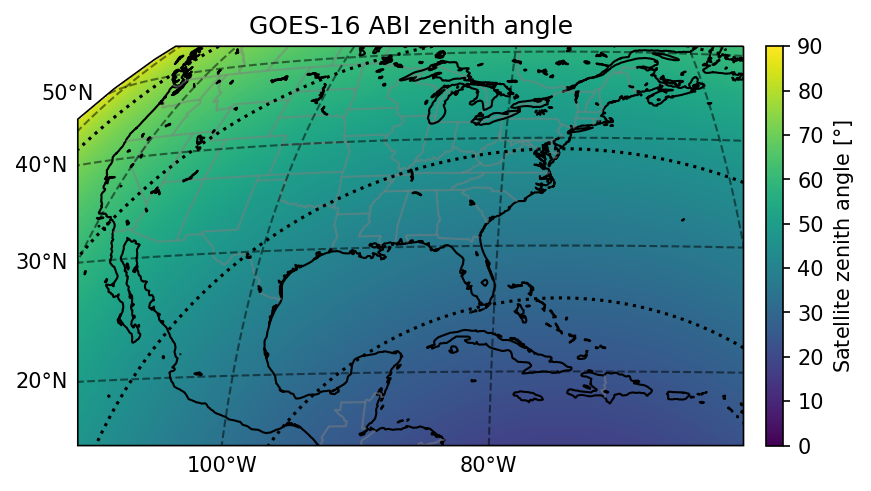
\includegraphics[width=\textwidth]{figures/ch2_01.png}
    \caption[
    The sensor zenith angle of \acrshort{goes}-16 \acrshort{abi} observations across the \acrshort{conus} domain
    ]{
    The sensor zenith angle of \acrshort{goes}-16 \acrshort{abi} observations across the \acrshort{conus} domain. Dotted arcs are shown for each 15\,\textdegree interval of zenith angle. Zenith angles in the north-west corner of the domain are particularly large, and so any observed \acrshort{dcc}s further north than 50\,\textdegree N or west of 120\,\textdegree W are removed from subsequent analysis.
    }
    \label{fig:abi_zenith_angles}
\end{figure}

To detect and track \acrshort{dcc}s across North America, we use \acrshort{abi} \acrshort{mcmip} data from the 6.2, 7.3, 10.4 and 12.4\,\unit{\mu m} channels observed in the \acrshort{conus} region, as described in section \ref{sec:abi_data}.
We use the full extent of the \acrshort{abi} \acrshort{conus} domain of 2,500~pixels E--W by 1,500~pixels N--S.
This domain covers a region of around 60--120\,\textdegree W in longitude and 15--60\,\textdegree N in latitude, covering an area of approximately 5,700 by 3,900\,\unit{km}.
Figure~\ref{fig:abi_zenith_angles} shows the satellite zenith angle of \acrshort{abi} observations across the \acrshort{conus} domain.
The large sensor zenith angles in the North-West of the domain may introduce large errors in the detection and tracking algorithm, so for the rest of this chapter we will only consider \acrshort{dcc}s detected east of 120\,\textdegree W and south of 50\,\textdegree N.
As the viewing angle increases detection and tracking become more difficult.
This is due to the confounding between vertical and horizontal motion, and also due to the area of each pixel increasing with the zenith angle.

Five full years of data---from the start of 2018 to the end of 2022---are used to produce a dataset of detected \acrshort{dcc}s and their properties.
This period spans all complete years of operational data from \acrshort{goes}-16 \acrshort{abi}.
To improve to continuity of observations, we then perform a gap-filling procedure.
If time gaps between observations of greater than 15 minutes are present we use observations from the full-disc \acrshort{abi} scan to fill these gaps.
Full disc imagery is typically available every 10 or 15 minutes depending on the operating mode.
This gap filling is particularly important during the periods in which \acrshort{abi} uses its mode 4 scan pattern, in which no \acrshort{conus} domain scans are made, but the full-disc is scanned every 5 minutes.
Using the full-disc observations allows us to maintain temporal sampling throughout these periods.


\section{Method}

Detection and tracking of convective cores and anvil cloud is performed using the method described in section~\ref{sec:tracking_method}.
Initial detection of \acrshort{dcc}s is performed separately over 24-hour periods spanning from 12:00:00~\acrshort{utc} (approximately 6am local time over North America) to the same time the next day.
This 24-hour period was dictated due to performance constraints, as the large domain combined with the high spatial and temporal resolution of \acrshort{abi} data results in a large memory requirement.
This time corresponds with the minima of convective activity over land, and so was chosen in order to minimise the number of \acrshort{dcc}s missed at the start and end of the detection period.
Each period is extended by six \acrshort{abi} observations at each end to ensure at least one hour of overlap between successive days.

To track long-lived \acrshort{dcc}s that last beyond one day, we apply a linking algorithm which combines \acrshort{dcc}s observed across multiple days.
The linking algorithm combines \acrshort{dcc}s detected at the same locations within the overlap period of two daily detection files.
Splitting and merging of objects is taken into account, so a single object which splits into two, or two objects which merge into one in the subsequent file are all considered a single, tracked object.
The linking algorithm is applied separately to each month of data for performance reasons.

After linking, a processing step is applied to calculate the properties of detected cores and anvils at each step of their lifecycles.
Finally, core and anvil step properties are aggregated over each month of observation, and overall core and anvil properties are calculated.
During this final step quality flagging is performed to isolate detected features that fail one or more quality checks.
The quality criteria are split into two criteria.
The first set of criteria---for core or anvil removal---removes detected features which should not pass the criteria for detection in the first place.
Detected features which flag any of these criteria are removed from the aggregated dataset in their entirety.
This step in particular removes anvils which have no cores associated with them, or are not detected as initiating with a developing core.

The second set of criteria is used to identify detected cores or anvils for which we do not observe their entire extent or lifecycle.
Cores and anvils which flag are of these criteria are still included within the aggregated properties dataset, but are not used when investigating \acrshort{dcc} properties throughout this chapter.

Quality criteria for cores are listed in table \ref{table:core_validity_criteria}, and those for anvils in table \ref{table:anvil_validity_criteria}.

%t
\begin{table}[tb]
\centering
\begin{tabular}{ll}
\tophline
Core removed if:                                                    & Core invalid if: \\
\middlehline
Initial \acrshort{bt} -- final \acrshort{bt} \textless~8\,\unit{K}  & Intersects edge of domain \\
Lifetime \textless~15~minutes                                       & Intersects start of domain \\
Time gaps \textgreater~15~minutes                                   & Intersects end of domain \\
Maximum area \textgreater~10,000\,\unit{km\textsuperscript{2}}      & Adjacent to bad \acrshort{abi} data \\
Any NaN values in core properties                                   & \\
\bottomhline
\end{tabular}
\caption[
Validity criteria for detected cores
]{
Validity criteria for detected cores. Cores which flag any of the removal criteria are removed in their entirety from the dataset. Those which flag any of the invalid criteria are retained, but removed from subsequent analysis.}
\label{table:core_validity_criteria}
\end{table}


%t
\begin{table}[tb]
\centering
\begin{tabular}{ll}
\tophline
Anvil removed if:                               & Anvil invalid if: \\
\middlehline
No associated cores                             & Intersects edge of domain \\
Lifetime \textless~15~minutes                   & Intersects start of domain \\             
Time gaps \textgreater~15~minutes               & Intersects end of domain \\
Maximum area \textless~maximum core area        & Adjacent to bad \acrshort{abi} data \\
Anvil detected before initial core              & Associated with invalid cores \\
Anvil dissipated before final core ends         & Maximum area reached before end \\
Any NaN values in anvil properties              & ~~of initial core \\
\bottomhline
\end{tabular}
\caption[
Validity criteria for detected anvils
]{
Validity criteria for detected anvil. Anvils which flag any of the removal criteria are removed in their entirety from the dataset. Those which flag any of the invalid criteria are retained, but removed from subsequent analysis. The majority of anvils removed are due to have no associated cores, or because the anvil was observed before any developing cores.}
\label{table:anvil_validity_criteria}
\end{table}


The complete processing pathway is outlined by the following steps:

\begin{enumerate}
    \item Detection of cores and anvils in \acrshort{abi} observations over each 24-hour period.
    \item Linking of overlapping objects detected in subsequent 24-hour periods over each month.
    \item Calculation of core and anvil step properties. 
    \item Quality criteria applied to core and anvils, properties aggregated over each month
\end{enumerate}

Two datasets are produced. The first consists of daily core and anvil spatial maps, with step properties, produced by processing step 3. 
The second, consisting of aggregated monthly core and anvil properties, is produced by step 4.

\begin{figure}[tp]
    \centering
    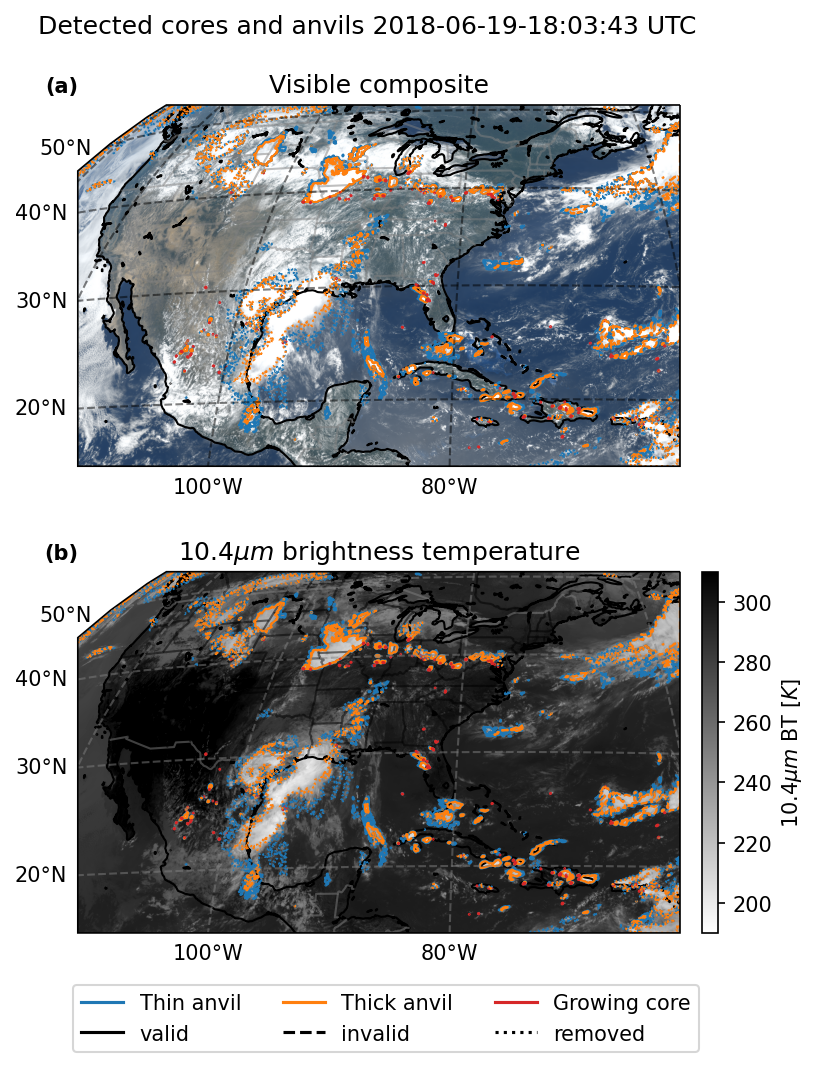
\includegraphics[width=\textwidth]{figures/ch2_02.png}
    \caption[
    Detected cores and anvils from a snapshot of \acrshort{goes}-16 \acrshort{conus} domain observations
    ]{
    Detected cores and anvils from a snapshot of \acrshort{goes}-16 \acrshort{conus} domain observations. Cores and anvils removed from the aggregated dataset are shown with dotted outlines. Those which are flagged as invalid are shown with dashed outlines. Detected features are shown against (a) visible composite imagery and (b) 10.4\,\unit{\mu m} \acrshort{bt}
    }
    \label{fig:conus_detected_dccs}
\end{figure}

Figure~\ref{fig:conus_detected_dccs} shows an example of detected cores and anvils over the \acrshort{conus} region, against backgrounds of composite visible imagery (fig.~\ref{fig:conus_detected_dccs}\,a) and 10.4\,\unit{\mu m} \acrshort{bt} (fig.~\ref{fig:conus_detected_dccs}\,b).
Cores and anvils which are removed from the aggregated dataset are outlined with dotted lines, and those which are marker invalid are shown with dashed outlines.

Over the five-year observing period we detect a total of 3,877,130 cores, of which 3,817,286 are valid, and 648,345 anvils, of which 576,555 are valid.


% \section{A novel method for detecting deep convective cloud cores and their associated anvils in geostationary satellite imagery}

% Numerous algorithms have been developed for the purpose of automatically detecting and tracking \acrshort{dcc}s, and are widely used for both forecasting and research purposes \citep[e.g.][]{mecikalski_use_2011, senf_characterization_2015, senf_satellite-based_2017, feng_life_2012, feng_spatiotemporal_2019, zinner_cb-tram:_2008}.
% Development of these algorithms has seen constant and continuous efforts.
% However a number of difficulties must be taken into account when utilising geostationary satellite imagery to detect and track \acrshort{dcc}s compared to the use of radar or lightning observations.


% Figure \ref{fig:compare_sat_radar_glm} provides an example of how geostationary satellite imagery compares to observations of \acrshort{dcc}s using ground-based cloud radar and lightning observations.
% In fig. \ref{fig:compare_sat_radar_glm}a, \ref{fig:compare_sat_radar_glm}d, \ref{fig:compare_sat_radar_glm}g and \ref{fig:compare_sat_radar_glm}e, we see how a growing \acrshort{dcc} is observed by visible/near infrared (NIR) satellite imagery, 10.4\,\unit{\mu m} longwave (LW) infrared (IR) satellite imagery, lightning flash observations from a satellite instrument and column radar reflectivity respectively.
% Figures \ref{fig:compare_sat_radar_glm}b, \ref{fig:compare_sat_radar_glm}e, \ref{fig:compare_sat_radar_glm}h and \ref{fig:compare_sat_radar_glm}k show observations of a mature \acrshort{dcc}, and \ref{fig:compare_sat_radar_glm}c, \ref{fig:compare_sat_radar_glm}f, \ref{fig:compare_sat_radar_glm}i and \ref{fig:compare_sat_radar_glm}l show those of a dissipating \acrshort{dcc}.
% While lightning and radar observations are capable of detecting deep convection in the growing and mature phase of \acrshort{dcc}s, neither can detect either the full extent of the anvil cloud or the dissipating phase of the \acrshort{dcc}.
% The ability to detect and track the anvil cloud over its entire lifetime is important to study the anvil cloud radiative forcing on the climate, the response to temperature change \citep{bony_thermodynamic_2016, hartmann_tropical_2016, ceppi_cloud_2017, gasparini_what_2019} and possible feedbacks on subsequent convective activity \citep{varble_erroneous_2018}.
% However, while radar and lightning observations of \acrshort{dcc}s can directly detect deep convection due to the strong correlations between core updraft intensity and radar reflectivity and polarisation \citep{austin_relation_1987, rosenfeld_general_1993, zipser_vertical_1994},  and lightning flash occurrence \citep{williams_relationship_1989, deierling_total_2008, wang_relationship_2017}, the same is not possible for geostationary satellite observations.
% Instead, a proxy variable linked to convective activity must be used to detect \acrshort{dcc}s.

% There are, in general, two approaches used as proxies for detecting convective clouds in geostationary satellite imagery. 
% Firstly, thresholds on observed field -- in particular LW IR brightness temperature (BT) -- are capable of detecting \acrshort{dcc} anvil clouds \citep[e.g.][]{schmetz_monitoring_1997, hong_detection_2005, schroder_deep_2009, liang_integrated_2017, senf_size-resolved_2018}.
% Secondly, the early stages of \acrshort{dcc}s can be detected using cloud top cooling rates \citep{zinner_cb-tram:_2008, bedka_objective_2010, muller_novel_2019}.
% The latter method is typically used for early detection of \acrshort{dcc}s for forecasting systems, as cloud top growth can detect \acrshort{dcc}s prior to radar observations \citep{roberts_nowcasting_2003}.
% While such algorithms provide an accurate detection of these early phases of \acrshort{dcc} growth \citep{zinner_validation_2013}, as the cooling of the cloud top is only visible during the initial phase of the \acrshort{dcc} any method that solely relies on detecting the growth of the \acrshort{dcc} will be unable to detect the anvil cloud after this initial growth phase has ended.

% On the other hand, threshold-based methods are better capable of detecting \acrshort{dcc}s throughout the mature phase, however are less able to detect the early stages of \acrshort{dcc} growth due to the inability to distinguish warm, growing \acrshort{dcc}s from other warm clouds.
% Furthermore, the choice of threshold value presents a limitation to the accuracy of threshold based detection methods.
% A choice of a warmer BT threshold results in false detections of non-convective clouds, whereas a colder threshold results in missed detections of \acrshort{dcc}s which do not meet the threshold, and further reduces the period over which \acrshort{dcc}s are detected.
% As the distributions of cloud top temperature for \acrshort{dcc}s and non-convective clouds overlap \citep{so_classification_2018}, there is no ideal threshold value that avoids this issue.
% \citet{fiolleau_algorithm_2013} implemented a single-step framework for detecting and tracking \acrshort{mcs}s that aims to address the compromise in detection accuracy by allowing a \acrshort{dcc} that is detected above a cold threshold BT at any time-step to be detected and tracked across the rest of its lifetime using a warmer threshold.
% Whereas this approach is successful for large, mesoscale systems, where the advection of the anvil is small compared to the over anvil area, it is less suitable for tracking small, rapidly moving convective cores due to the overlap between the spacing of neighbouring \acrshort{dcc} cores and the typical distance moved by cores between time steps \citep{heikenfeld_tobac_2019}.
% To improve the tracking of small \acrshort{dcc}s, we have developed a novel method which uses semi-Lagrangian framework for single-step detection and tracking which accounts for the motion of \acrshort{dcc}s using optical flow.
% This method allows us to first detect growing \acrshort{dcc} cores using a growth-based detection method, and then detect their associated anvil clouds even after growth is no longer detected.
% This method allows new capabilities in detected \acrshort{dcc}s over their entire lifecycles.

% \subsection{Overview of detection and tracking method}

% We present here an overview of the detection and tracking method presented in \citet{jones_semi-lagrangian_2022}.
% This method can be outlined in the following steps:

% \begin{itemize}
%     \item Ingest of LW IR BT fields from geostationary satellite imagery, and calculation of water vapour difference (WVD) and split window difference (SWD) fields.
%     \item Calculation of optical flow vectors to be used as an \textit{a priori} estimate of cloud motion for use in the semi-lagangian framework.
%     \item Detection of growing \acrshort{dcc} cores using cloud top cooling rate.
%     \item Detection of thick and thin anvil clouds associated with detected cores using a semi-lagrangian "3d" watershedding method. 
%     \item Grouping of cores into multi-core systems, calculation of statistics and validation using lightning observations.
% \end{itemize}

% \subsection{Data}

% The Advanced Baseline Imager (ABI), a radiometer aboard the Geostationary Operational Environmental Satellite (GOES)-16 weather satellite \citep{schmit_closer_2016}, provides visible and IR imagery at a nadir resolution of 2\,\unit{km} or better, at intervals between 10 minutes to 30 seconds \citep{schmit_chapter_2020}.
% Situated in a geostationary orbit at 75.2°W above the equator, GOES-16 observes all of South America and most of North America.
% The combination of high spatial and temporal resolution makes ABI suitable for detecting and tracking small and developing \acrshort{dcc}s, as well as providing the spatial coverage to also track large mesoscale convective systems \citep{heikenfeld_tobac_2019}.
% In addition, the better signal to noise ratio of ABI observations compared to previous geostationary imaging instruments \citep{iacovazzi_goes-16_2020}, combined with many of the channels being derived from those aboard the Visible Infrared Imaging Radiometer Suite (VIIRS), make the data from ABI better suited for research purposes than that from older instruments \citep{heidinger_chapter_2020}.

% In this paper we have used the ABI level 2 multi-channel cloud and moisture imagery product (MCMIP) over the continental US domain \citep{schmit_chapter_2020}.
% This product consists of calibrated reflectances and brightness temperatures on a common grid.
% All data has been sourced through the National Oceanic and Atmospheric Administration Big Data Program.

% In order to have equal performance during both day and nighttime, a selection of longwave IR ABI channels are used for the detection and tracking of \acrshort{dcc}s (see figure \ref{fig:abi_channels}). 
% These channels consist of the LW clean and dirty window channels at 10.4\,\unit{\mu m} and 12.4\,\unit{\mu m} respectively, and the upper and lower troposphere water vapour channels at 6.2\,\unit{\mu m} and 7.3\,\unit{\mu m} respectively.
% Whereas the LW window IR brightness temperature is commonly used for the detection of \acrshort{dcc}s, we have decided not to use it for this purpose in this method due to the wide range of brightness temperatures observed within anvil clouds, and the variance of anvil cloud temperature because of changes in tropopause temperature due to meteorology and latitude.
% However, the information contained within this field is used to for the optical flow calculation of the cloud motion field.

% Two additional combinations of channels are used to detect areas of deep convective cloud anvil. 
% The water vapour difference (WVD) combination (figure \ref{fig:abi_channels}b) of the upper troposphere WV channel minus the lower troposphere WV channel has been shown to provide a high detection rate for deep convective clouds \citep{muller_role_2018, muller_novel_2019}.
% In clear sky or low cloud conditions, WVD shows the temperature difference between the upper and lower troposphere of generally around -20 K. 
% However, in the presence of high, thick clouds the 6.2\,\unit{\mu m} has an additional contribution from stratospheric water vapour produces a warm, and in extreme cases positive WVD value \citep{schmetz_monitoring_1997}.
% This provides clear distinction between thick, high cloud and other clouds, with the cutoff value of -5 °C giving a high detection rate of anvil clouds \citep{muller_novel_2019}. 
% Furthermore, as the WVD values are relative to the lower stratosphere temperatures, this field is much less affected by location and meteorology than the LW IR channel.
% However, the WVD is still prone to the false detections of non-convective clouds when using a thresholding method.

% The split window difference (SWD) (figure \ref{fig:abi_channels}c) (the clean IR window channel minus the dirty IR window channel) aids in the detection and separation of optically thin anvil cloud (including cirrus outflow) from optically thick anvil due to the difference in ice particle emissivity between these two channels \citep{heidinger_gazing_2009}.
% As a result, this combination displays warm temperatures of around 10\,\unit{K} for thin, ice clouds, near 0\,\unit{K} for thick clouds, and approximately 5\,\unit{K} for clear skies due to the contribution of boundary layer water vapour.
% The SWD is, however, also sensitive to low level clouds and low level water vapour concentrations, and so cannot be used alone to detect \acrshort{dcc}s.
% The SWD field is useful, however, due to the difficulty in separating anvil clouds from cirrus when using LW IR BT alone \citep{hong_detection_2005}. 
% By subtracting the SWD from the WVD field, we can reduce the sensitivity of our detection scheme to cirrus clouds, reducing the rate of erroneous detections.
% Further, adding the SWD field to WVD field can enhance the appearance of cirrus, enabling the detection of cirrus outflow  from \acrshort{dcc} anvils.

% \subsection{Classification of \acrshort{dcc} cores and anvils}

% The detection and classification of \acrshort{dcc}s occurs over three steps.
% First, the cores are detected using regions of cooling cloud top BT.
% \citet{roberts_nowcasting_2003} identified cloud top cooling rates of between 4 and 8\,\unit{K} over a 15 minute period as being associated with weak convection, and greater than 8\,\unit{K} as associated with more intense convective development.
% Here we use corresponding threshold values of 0.25 and 0.5\,\unit{K minute\textsuperscript{-1}} respectively to detect developing deep convective cores.
% If we assume that the cloud top temperature of a growing \acrshort{dcc} core follows the moist pseudo-adiabat then this upper bound is equivalent to a cloud top vertical velocity of approximately 1.5\,\unit{ms\textsuperscript{-1}}.
% It should be made clear that this is not the same as the vertical velocity of the updraft within the core, and it is expected that the cloud top growth will be slower due to the impacts of entrainment on the growing cloud.

% A core is defined as a region of continuous cooling BT exceeding 0.25\,\unit{K minute\textsuperscript{-1}}, with at least one time step with as cooling rate greater than 0.5\,\unit{K minute\textsuperscript{-1}}.
% Several further constraints are applied to the detection of growing cores.
% First, a core must exist for at least 15 minutes.
% Secondly, the core must reach a WVD of greater than -5\,\unit{K}, the criteria used by \citet{muller_role_2018} to detect high, thick clouds.
% The challenge of detecting changes in BT due to vertical cloud growth, rather than that due to horizontal motion or growth of the anvil cloud \citep{hartung_intercomparison_2013}, is handled by using the semi-lagrangian framework to account for cloud motion when calculating the change in BT over time.
% Furthermore, a curvature filter is used to isolate growth only in regions that display a peak of cold BT, in order to prevent erroneous detections of cloud growth in regions where multiple clouds and merging together.
% When calculating the BT cooling rate, the WVD field, rather than LW IR window BT, is used as this is only sensitive to mid- and upper-level growth associated with deep convection.

% Following core detection, the associated anvil cloud is detected using a "3d" watershed approach in the same manner as \citet{fiolleau_algorithm_2013}.
% Rather than use BT thresholds for detecting the anvil cloud, we use the detected core regions as the seed for the watershedding, and use an edge detection method to detect the extent of the anvil cloud as used by \citet{dim_alternative_2013}.
% By using the detected core regions as the initial seed for the watershed segmentation, we only detect anvil clouds that are associated with detected regions of convective growth.
% Utilising the semi-Lagrangian scheme to account for cloud motion, we can apply the "3d" watershedding method to cases of small, rapidly moving cores and anvils where previously this approach would not be applicable.
% Use of the edge detection method allows us to avoid the use of a fixed threshold and instead detect the full extent of the anvil cloud while avoiding the challenges of warm BT thresholds previously discussed.
% To detect the region of thick anvil cloud associated with cores, the edge detection method is applied to the WVD field minus the SWD field (to remove thin cirrus), with edges detected in the range of -5 and -15\,\unit{K}.
% A detected thick anvil cloud may be associated with multiple cores, allowing us to detect cases where the multiple \acrshort{dcc}s have merged into one.
% Finally, we detect the thin anvil region -- including cirrus outflow -- by repeating the procedure for detecting the thick anvils but instead using the WVD field plus the SWD field for edge detection.
% This allows us to detect thin, high level clouds that are associated with detected cores and anvils without detecting isolated cirrus.

% Figure \ref{fig:detected_anvils} shows an example of the results of detecting and tracking \acrshort{dcc} cores and their associated anvils.
% Detection of the cores (outlined in red) and the initial development of the associated anvils (outlined in orange and blue for the thick and thin anvil regions respectively) can be seen in figure \ref{fig:detected_anvils}a.
% In figure \ref{fig:detected_anvils}b we see the development of the mature anvil, which primarily consists of thick anvil, and secondary core detections as new convection develops at the edge of the \acrshort{dcc}.
% In figure \ref{fig:detected_anvils}c, we see the detected anvil cloud begin to dissipate, with a larger proportion of the anvil cloud detected as thin anvil.
% It should be noted that the algorithm is capable of tracking both individual cores and their associated anvil clouds, including when multiple cores feed into a single anvil.
% Furthermore, the anvil cloud and the outflow region continue to be tracked after growing cores can no longer be detected.

% In this study, we have generated a dataset of detected cores and their associated anvil clouds for a subset of the GOES-16 CONUS region spanning from 114 to 76\textdegree~W and from 24 to 45\textdegree~N, an area of approximately 2,500 by 1,875\,\unit{km}, for the entirety of the year 2018.
% Days were excluded from the dataset when there were periods of missing data exceeding 15~minutes or when anomalies in the ABI data that may have affected core or anvil detection were present.
% In total, this removed 35~days, resulting in the remaining dataset covering 330~days of 2018.

% In total, over the course of 2018, we detected 80,644 unique cores and 22,526 unique anvils.
% Of these, 1,592 cores and 7,992 anvils were detected intersecting the edge of the domain and have been removed from analysis of the properties and lifetimes of cores and anvils to avoid incomplete data.
% Due to technical limitations for processing the long time series of data, no anvils are detected with a lifetime of over 24~hours.
% We plan in future to address this issue in order to detect long lived \acrshort{dcc}s.

\section{Results}


\subsection{Temporal and spatial distributions of detected cores over North America} \label{sec:core_properties}


%f
\begin{figure}[tp]
    \centering
    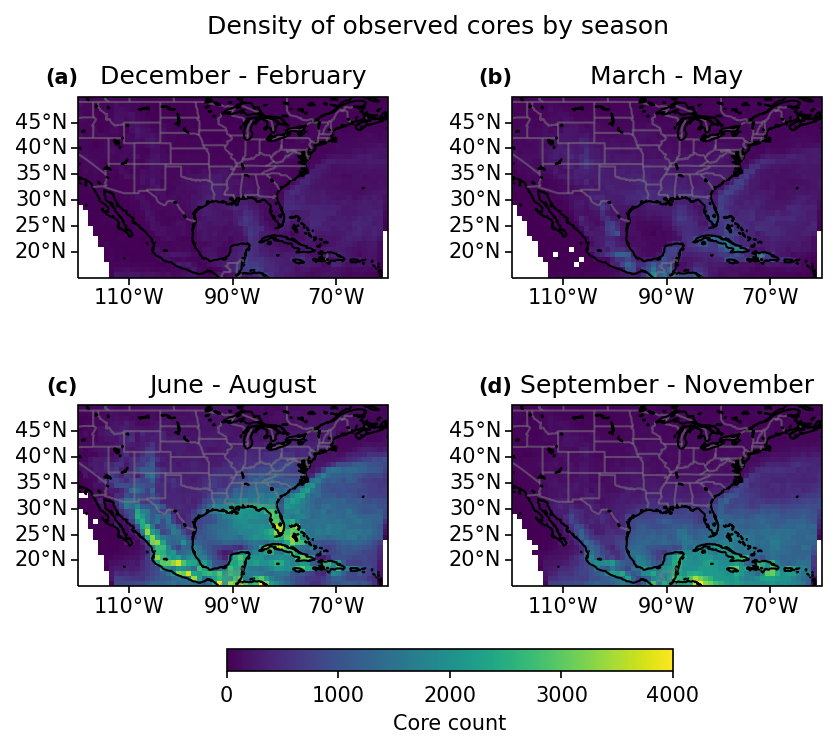
\includegraphics[width=\textwidth]{figures/ch2_03.png}
    \caption[
    The spatial distribution of observed cores by season
    ]{
    The spatial distribution of observed cores, broken down by season and accumulated into 1\texttimes1\textdegree\ grid boxes of latitude and longitude. The density of observed cores is greatest during summer (c) and smallest during winter (a).
    }
    \label{fig:core_density_by_season}
\end{figure}

To begin, we investigate the distribution of detected \acrshort{dcc} cores throughout the dataset.
In fig.~\ref{fig:core_density_by_season} we plot the distribution of observed cores over North America separated by season.
Large variations in the spatial distribution of cores can be observed across the different seasons.
Overall, in winter and spring (fig.~\ref{fig:core_density_by_season}\,a,b) we see lower rates of the observed \acrshort{dcc}s than in the summer and autumn (fig.~\ref{fig:core_density_by_season}\,c,d).

In winter (fig.~\ref{fig:core_density_by_season}\,a) the majority of convection observed occurs over the ocean, particularly in the areas of the Gulf of Mexico and West Atlantic associated with warm currents.
In spring (fig.~\ref{fig:core_density_by_season}\,b) we see a similar pattern over ocean, however there is also an increase in convection detected over land in the Caribbean, Mexico and the central and southern \acrshort{usa}.
In summer (fig.~\ref{fig:core_density_by_season}\,c) we a large increase in convection over land and ocean, with the highest rates of convection of any season.
In particular we see high rates of convection over Mexico, the Caribbean, the southern \acrshort{usa} (Florida in particular) and adjacent ocean regions.
In Autumn (fig.~\ref{fig:core_density_by_season}\,d), we see a large reduction in the number of convective cores detected over land regions.
The number of detections over the ocean remains high however, indicating a possible lag in the seasonal cycle of convection over oceans compared to that over land.

%f
\begin{figure}[tp]
    \centering
    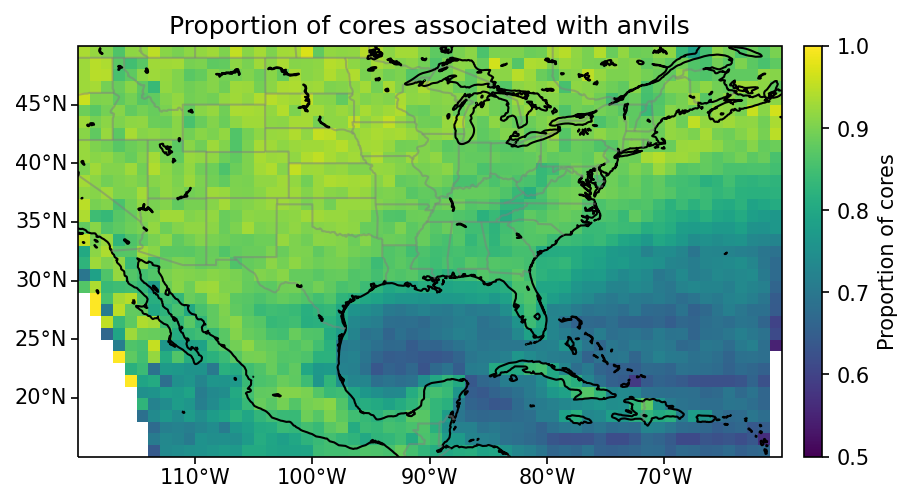
\includegraphics[width=\textwidth]{figures/ch2_04.png}
    \caption[
    The proportion of detection cores associated with anvils
    ]{
    The proportion of detection cores associated with anvils in each 1\texttimes1\textdegree\ grid box. In general, we see that the majority of cores over land are associated with anvils, while over the ocean a larger number are detected without anvils.
    }
    \label{fig:cores_with_anvils_map}
\end{figure}

Figure~\ref{fig:cores_with_anvils_map} shows the proportion of cores associated with anvil clouds.
We see a clear land--sea contrast, with a much larger number of cores occurring without associated anvil clouds over the ocean than over land.

%f
\begin{figure}[tp]
    \centering
    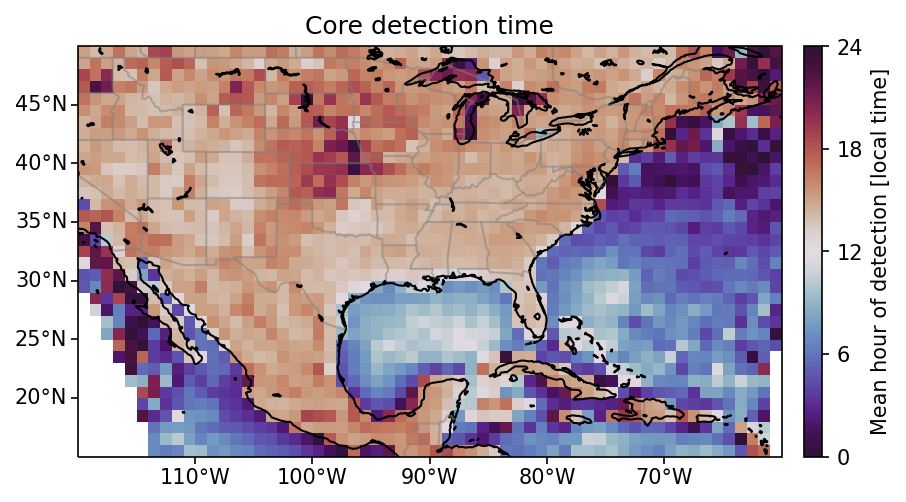
\includegraphics[width=\textwidth]{figures/ch2_05.png}
    \caption[
    The average time of initiation of observed cores
    ]{
    The average time of day of initiation of cores observed within each 1\texttimes1\textdegree\ grid box. The time of initiation is calculated as the local solar time based on longitude, and the mean is calculated as the circular mean to account for the cyclical aspect of the hour of day.
    }
    \label{fig:core_detection_time_map}
\end{figure}

In fig.~\ref{fig:core_detection_time_map}, we show the mean time of detection for cores detected within each 1-degree grid square.
The most notable feature in fig.~\ref{fig:core_detection_time_map} is the strong land-sea contrast, with the majority of land regions showing convective activity occurring during the afternoon, and the majority of ocean regions showing activity before midday.
In addition, we see a few major features of the detected time of initiation across both land and sea regions.

In coastal regions in the Gulf of Mexico and the Caribbean Sea, we see earlier initiation times closer to coastlines, while regions further from land have average times of detection closer to midday.


Over the land, we see a later time of initiation over the Northern Great Plains (90--100\,\textdegree W, 37--47\,\textdegree N).

% \subsubsection{Regional differences in the time of core detection}

%f
\begin{figure}[tp]
    \centering
    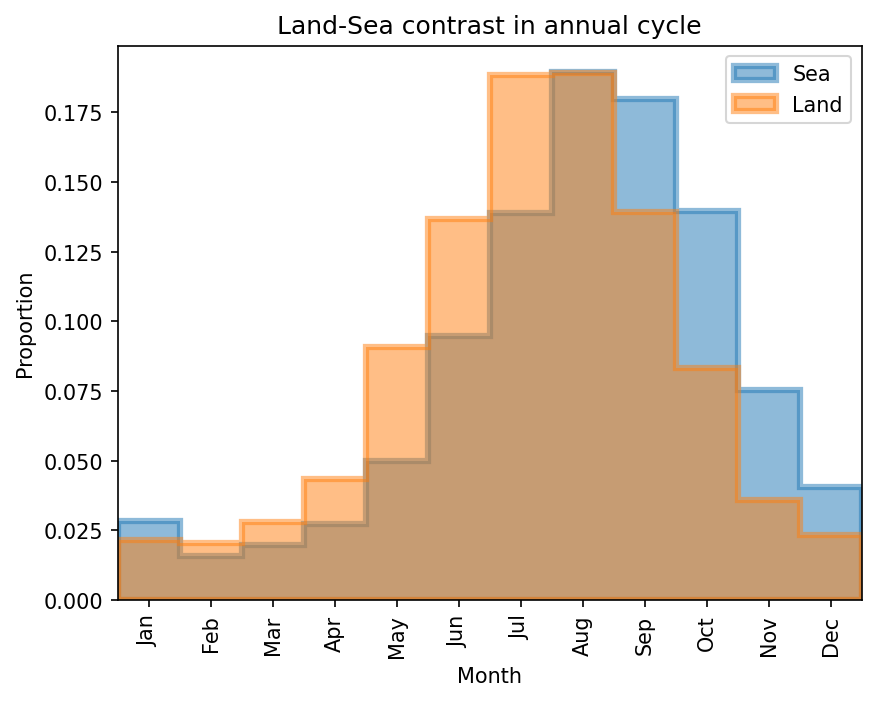
\includegraphics[width=\textwidth]{figures/ch2_land_sea_monthly.png}
    \caption[
    Monthly distributions of the proportion of cores detected each month for land and sea regions
    ]{
    Monthly distributions of the proportion of cores detected each month for land and sea regions.
    }
    \label{fig:core_annual_land_sea}
\end{figure}

Figure~\ref{fig:core_annual_land_sea} shows the proportion of cores detected in each month over the annual cycle for land and sea regions.
Both land and sea regions show a peak of convective activity in the summer, and a low in the winter months.
However, as suggested by fig.~\ref{fig:core_density_by_season}, there is a time lag of about 1 month between the annual cycle of convection over land and that over ocean, likely due to the time lag in ocean heating.

%f
\begin{figure}[tp]
    \centering
    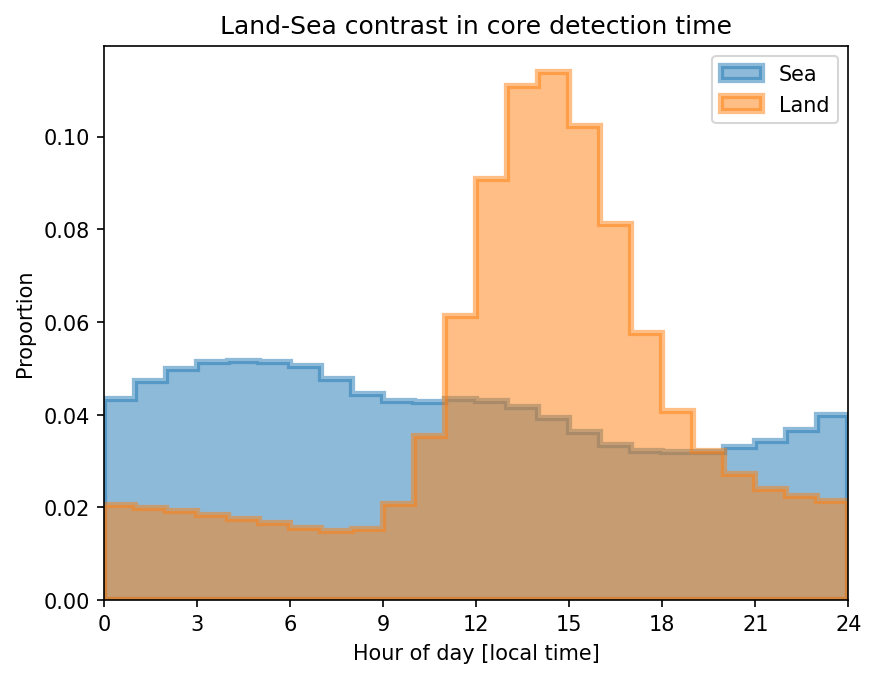
\includegraphics[width=\textwidth]{figures/ch2_land_sea_diurnal.png}
    \caption[
    The diurnal distributions of the local time of detection for cores detected over land and sea
    ]{
    The diurnal distributions of the local time of detection for cores detected over land and sea.
    }
    \label{fig:core_diurnal_land_sea}
\end{figure}

Figure~\ref{fig:core_diurnal_land_sea} shows the distribution of core detections across the diurnal cycle for land and sea regions.
Unlike in fig.~\ref{fig:core_annual_land_sea}, we see a large difference in the shape of the two distributions.
Over land, we see a sharp peak in convective activity occurring in the mid afternoon, with a tail extending into the night-time.
Over the sea the distribution of core detections is much more uniform across the diurnal cycle.
There is still a peak observed in the early hours of the morning (3--6\,am), and a low in the evening (6\,pm), but the difference between these is much less pronounced than that over land.

%f
\begin{figure}[tp]
    \centering
    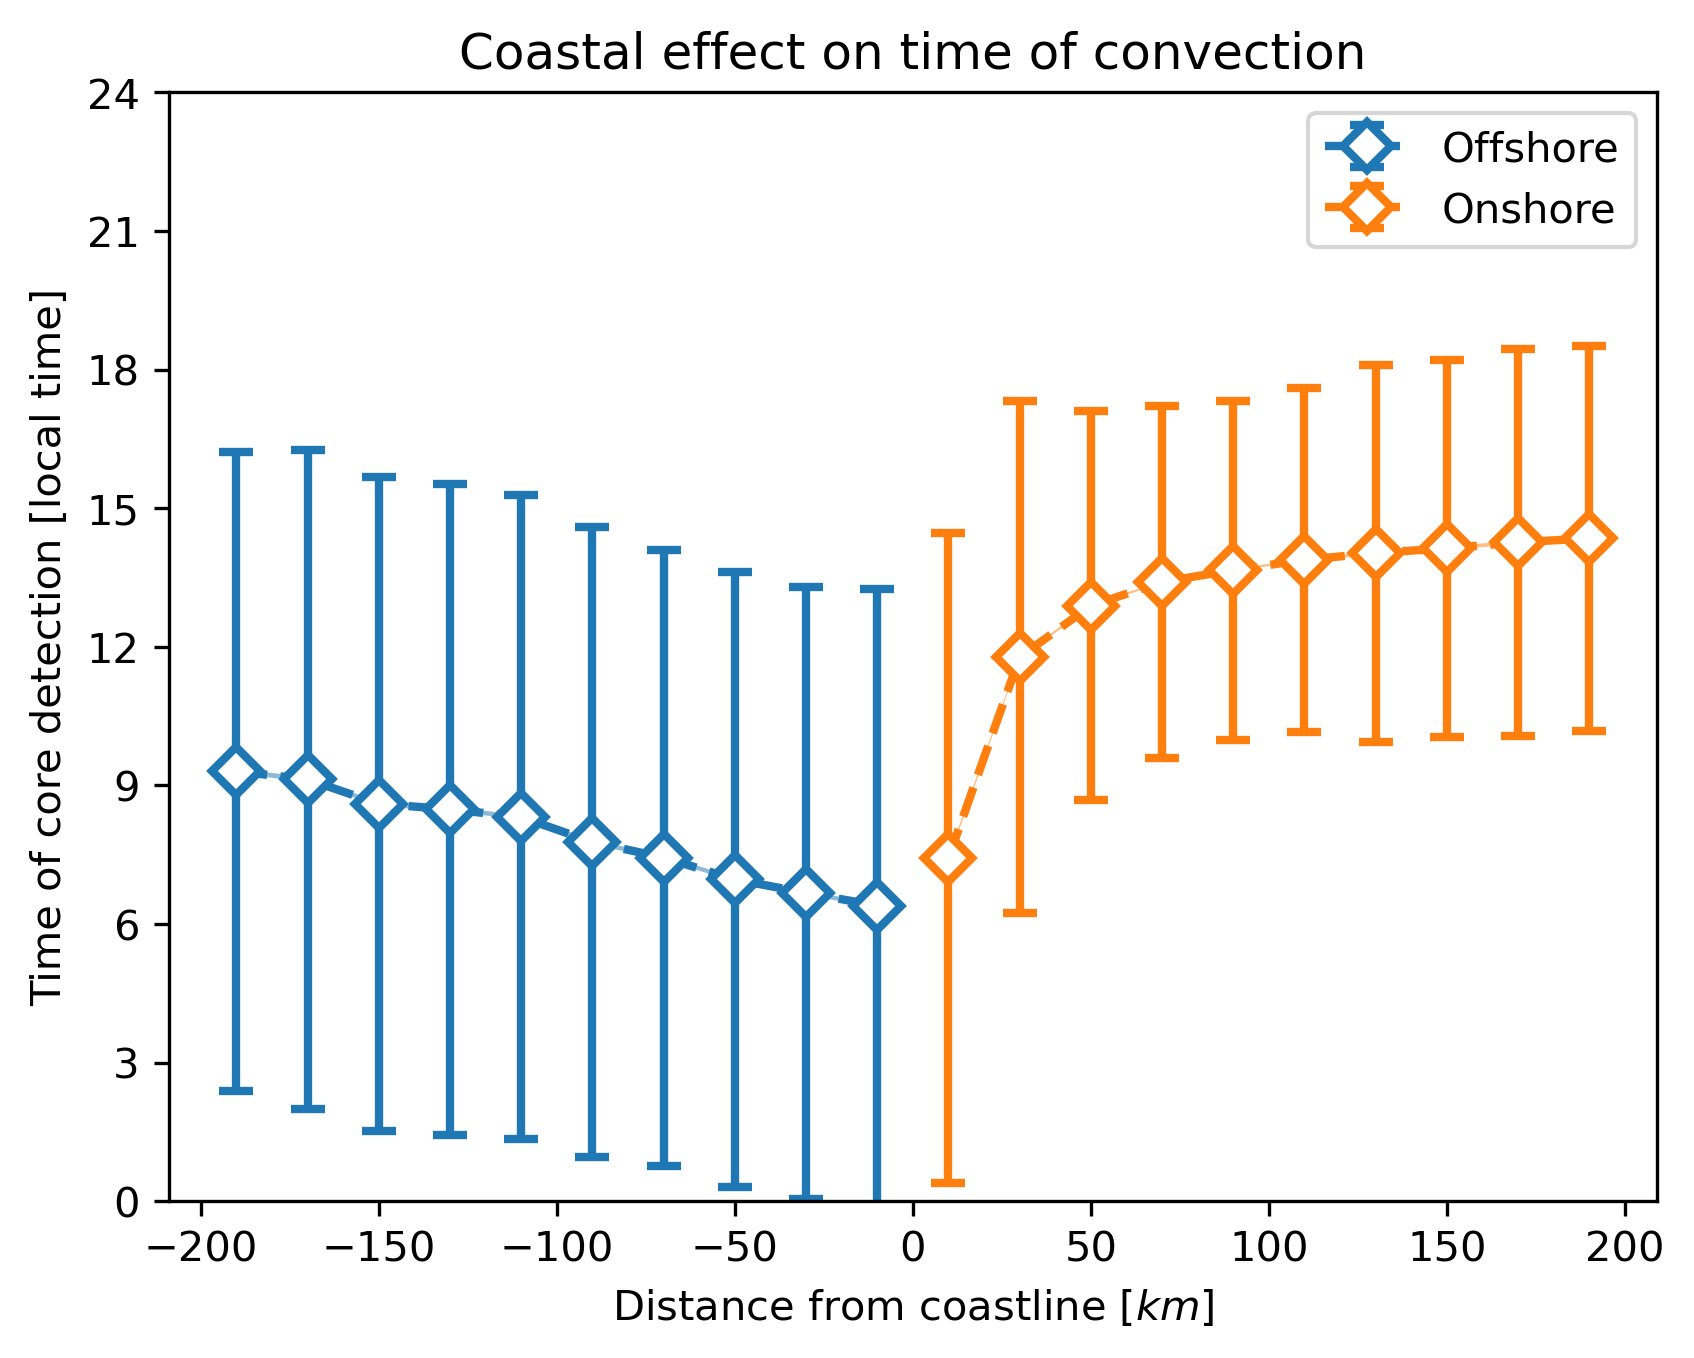
\includegraphics[width=\textwidth]{figures/ch2_coastal_effect.png}
    \caption[
    The change in average time of core detection with distance from the coastline
    ]{
    The change in average time of core detection with distance from the coastline.
    }
    \label{fig:core_coast_effect}
\end{figure}

In fig.~\ref{fig:core_coast_effect} we examine the effect of the distance to the coast on core detection time over the Gulf Coast region (22.5--32.5\,\textdegree\,N, 82.5--100\,\textdegree\,W).
Negative distances indicate locations further offshore, and positive distances those locations further inland.
In fig.~\ref{fig:core_detection_time_map} we saw a change in the average time of detection of cores in locations closer to the coast, and that effect is shown again here.
For cores detected over sea, we see a linear decrease in the average time of detection as the distance to the coast increases.
For cores detected over land, we see a sharp decrease in the time of detection very close to the coast, however further than 50\,\unit{km} from the coast this becomes a shallower linear gradient.
The linear change of core detection time with distance from the coastline may be linked to offshore and onshore breezes triggering convection.
For cores over land, we see a reduction in the variance of the time of detection between 50 and 120\,\unit{km} from the coast, which may also indicate that an external forcing from sea breeze is triggering convection in these areas, and hence constraining the time of initiation of convection.

%f
\begin{figure}[tp]
    \centering
    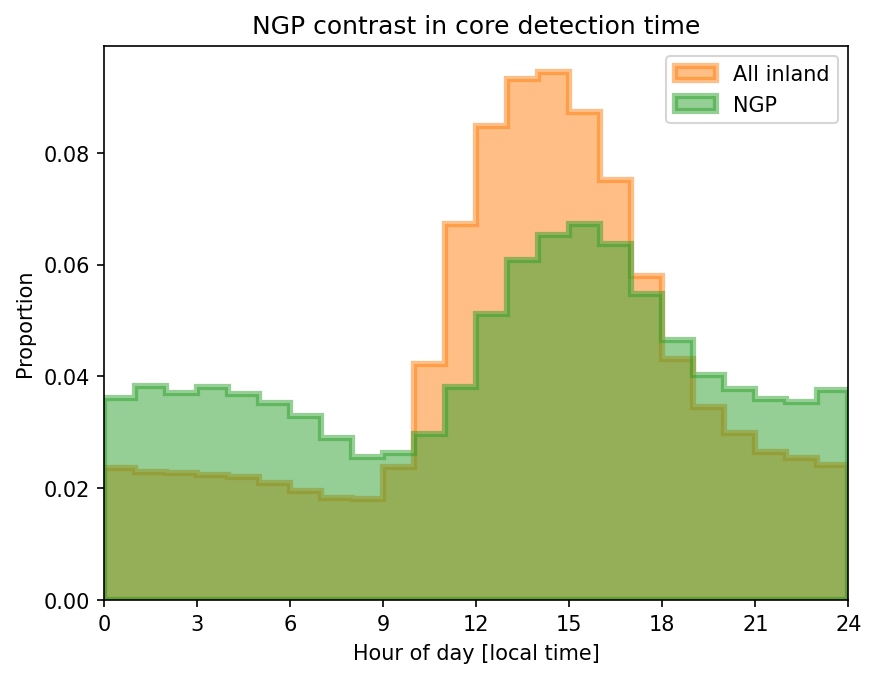
\includegraphics[width=\textwidth]{figures/ch2_NGP_diurnal.png}
    \caption[
    A comparison of the diurnal distribution of cores detected in the \acrshort{ngp} region with all extra-tropical land regions
    ]{
    A comparison of the diurnal distribution of cores detected in the \acrshort{ngp} region with all extra-tropical land regions.
    }
    \label{fig:core_ngp_contrast}
\end{figure}

In fig.~\ref{fig:core_detection_time_map} we saw a noticeably later average time of detection over the \acrshort{ngp} region.
Figure~\ref{fig:core_ngp_contrast} shows how the diurnal distribution of core detection time varies compared to that over all extra-tropical land regions (defined as \textgreater\,30\,\textdegree\,N and \textgreater\,200\,\unit{km} away from a coastline).
For all inland cores, we see a sharp peak in the early afternoon similar to that for all land in fig.~\ref{fig:core_diurnal_land_sea}, albeit with reduced contrast between the peak and nighttime.
In contrast, the \acrshort{ngp} region shows a later peak of convective activity as well as much higher rates of convection observed during the nighttime and into the early morning, with a secondary, wider peak between midnight and 5\,am.
This mirrors the results of \citet{li_high-resolution_2021}, who found a similar bimodal distribution in convective precipitation over the \acrshort{ngp}


% \subsubsection{Regional core dynamics}

%f
\begin{figure}[tp]
    \centering
    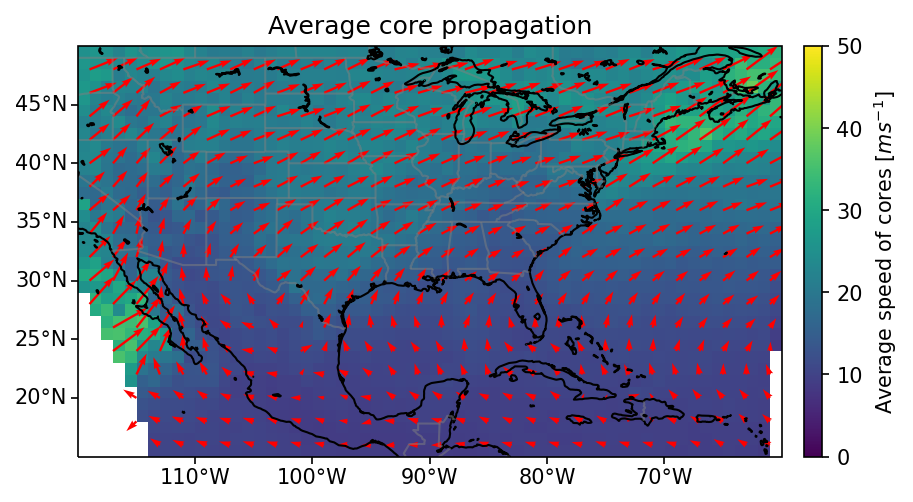
\includegraphics[width=\textwidth]{figures/ch2_06.png}
    \caption[
    The average speed and direction of propagation of cores
    ]{
    The average speed and direction of propagation of cores observed within each 1\texttimes1\textdegree\ grid box. The colouring shows the average speed of propagation, and the red arrows show the average direction for each 2\texttimes2\textdegree\ grid box}
    \label{fig:core_propagation_map}
\end{figure}

Figure~\ref{fig:core_propagation_map} shows the average speed of propagation for cores observed in each 1-degree grid box, with the average direction of propagation shown by arrows for each 2-degree grid box.
We see a clear change in the direction of propagation from an easterly motion in the tropics (below 25\,\textdegree N) to a westerly motion in the mid-latitudes.


In the following two figures (fig.~\ref{fig:core_lifetime_map} and \ref{fig:core_cooling_rate_map} we only map the properties of cores which initiate with an average brightness temperature of greater than 273\,\unit{K}.
This is done to show the average properties of cores which we observe developing in clear sky or low cloud conditions, and exclude those which form within existing anvil clouds.
This shows where we expect to observe the full lifetime of the observed core.

%f
\begin{figure}[tp]
    \centering
    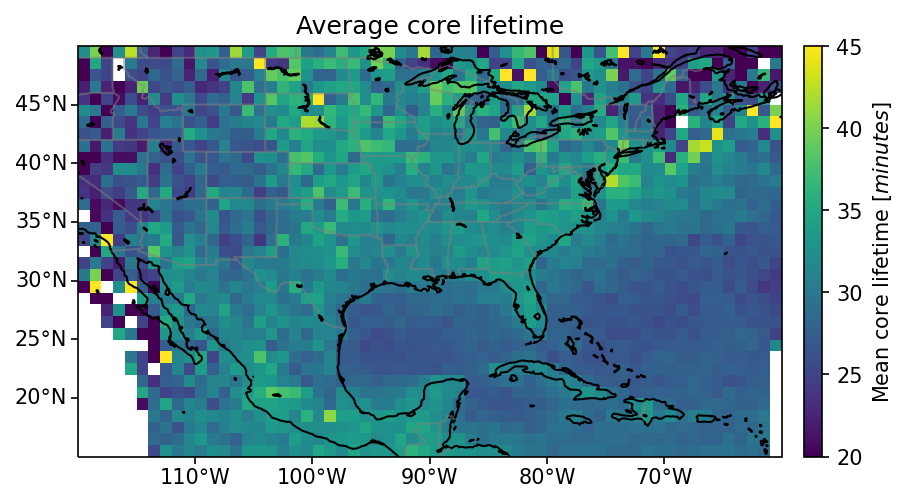
\includegraphics[width=\textwidth]{figures/ch2_07.png}
    \caption[
    The mean lifetime in minutes of cores
    ]{
    The mean lifetime in minutes of cores within each 1\texttimes1
    \textdegree\ grid box.
    }
    \label{fig:core_lifetime_map}
\end{figure}

Figure \ref{fig:core_lifetime_map} displays the mean lifetime of observed cores over each 1-degree box of latitude and longitude.
We see a contrast between land and sea, with cores occurring over the ocean having a shorter lifetime, and an increase in the average core duration over the Great Plains region.

%f
\begin{figure}[tp]
    \centering
    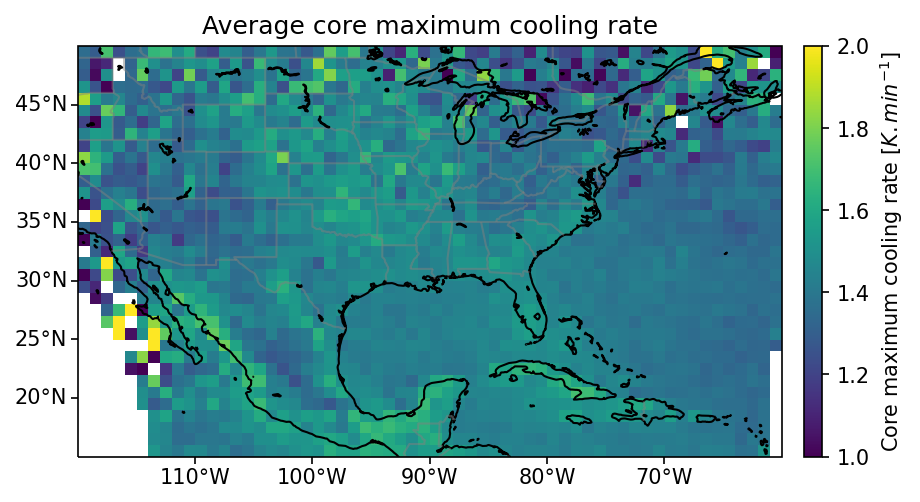
\includegraphics[width=\textwidth]{figures/ch2_08.png}
    \caption[
    The average maximum core cooling rate
    ]{
    The average maximum core cooling rate for each 1\texttimes1
    \textdegree\ grid box.
    }
    \label{fig:core_cooling_rate_map}
\end{figure}

Figure~\ref{fig:core_cooling_rate_map} shows the average cooling rate of observed cores.
Some contrast is seen again between land and sea, particularly in the Caribbean, but this is less pronounced than the difference in lifetime shown in fig.~\ref{fig:core_lifetime_map}.


% \subsubsection{Relations between the properties of developing cores}

%f
\begin{figure}[tp]
    \centering
    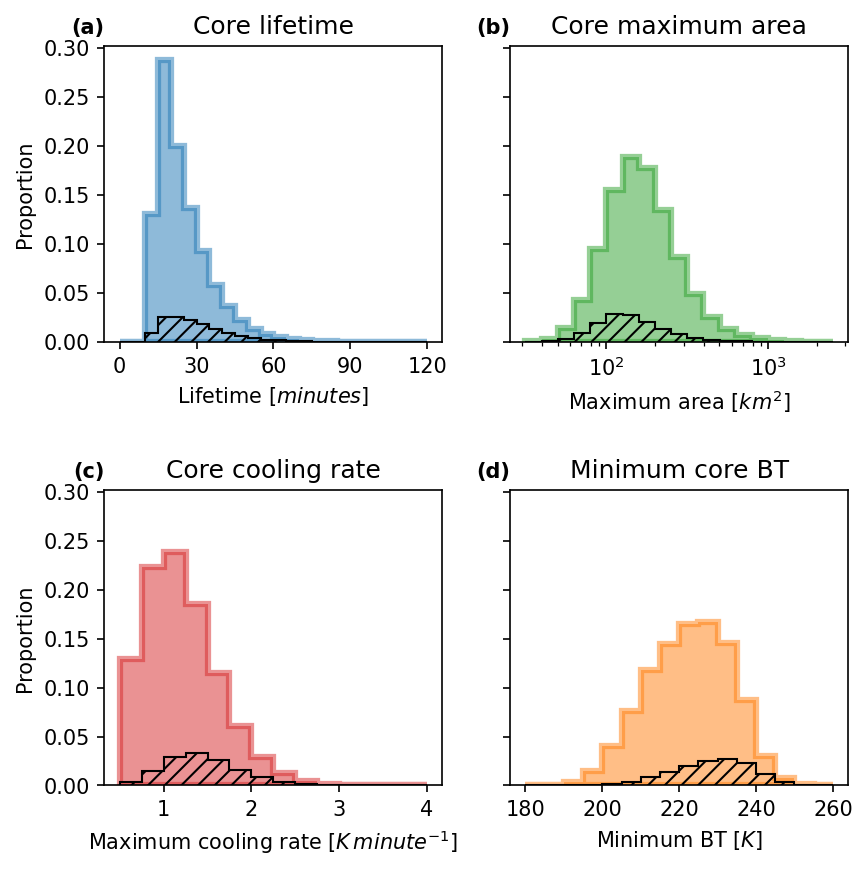
\includegraphics[width=\textwidth]{figures/ch2_09.png}
    \caption[
    Histograms showing the distributions of observed core properties
    ]{
    Histograms showing the distributions of observed core lifetime (a), maximum area (b), maximum cooling rate (c) and minimum \acrshort{bt} (d). The hatched areas show the proportion of each distribution consisting of cores which were detected with an initial average \acrshort{bt} less than 273\,\unit{K}.
    }
    \label{fig:core_properties}
\end{figure}

Figure~\ref{fig:core_properties} shows the distributions of lifetime (fig.~\ref{fig:core_properties}\,a), maximum area (fig.~\ref{fig:core_properties}\,b), cooling rate (fig.~\ref{fig:core_properties}\,c) and minimum \acrshort{bt} (fig.~\ref{fig:core_properties}\,d).
The hatched areas show the distributions of cores with warm initial \acrshort{bt}.
In general, cores observed with warm initial \acrshort{bt} tend to have longer lifetimes and greater cooling rates.
However, they also tend to have smaller maximum areas and warmer minimum \acrshort{bt}, indicating that cores observed forming within existing anvil clouds tend to have both larger areas and colder \acrshort{bt}.

Figure~\ref{fig:core_cooling_rate_relations}\,a compares how the average lifetime of detected cores changes with their maximum observed cooling rate.
For low values of core cooling rate, we see a similar, positive linear relationship between cooling rate and lifetime between all regions, indicating that more intense convection leads to longer periods of cores being observed.
However, beyond cooling rates of around 1.5\,\unit{K minute\textsuperscript{-1}} we see an inflexion in the relationship, with larger cooling rates leading to shorter lifetimes.
This may be explained by the cores with faster cooling rates reaching their level of neutral buoyancy faster, and therefore showing cooling cloud tops for a shorter period of time.

%f
\begin{figure}[tp]
    \centering
    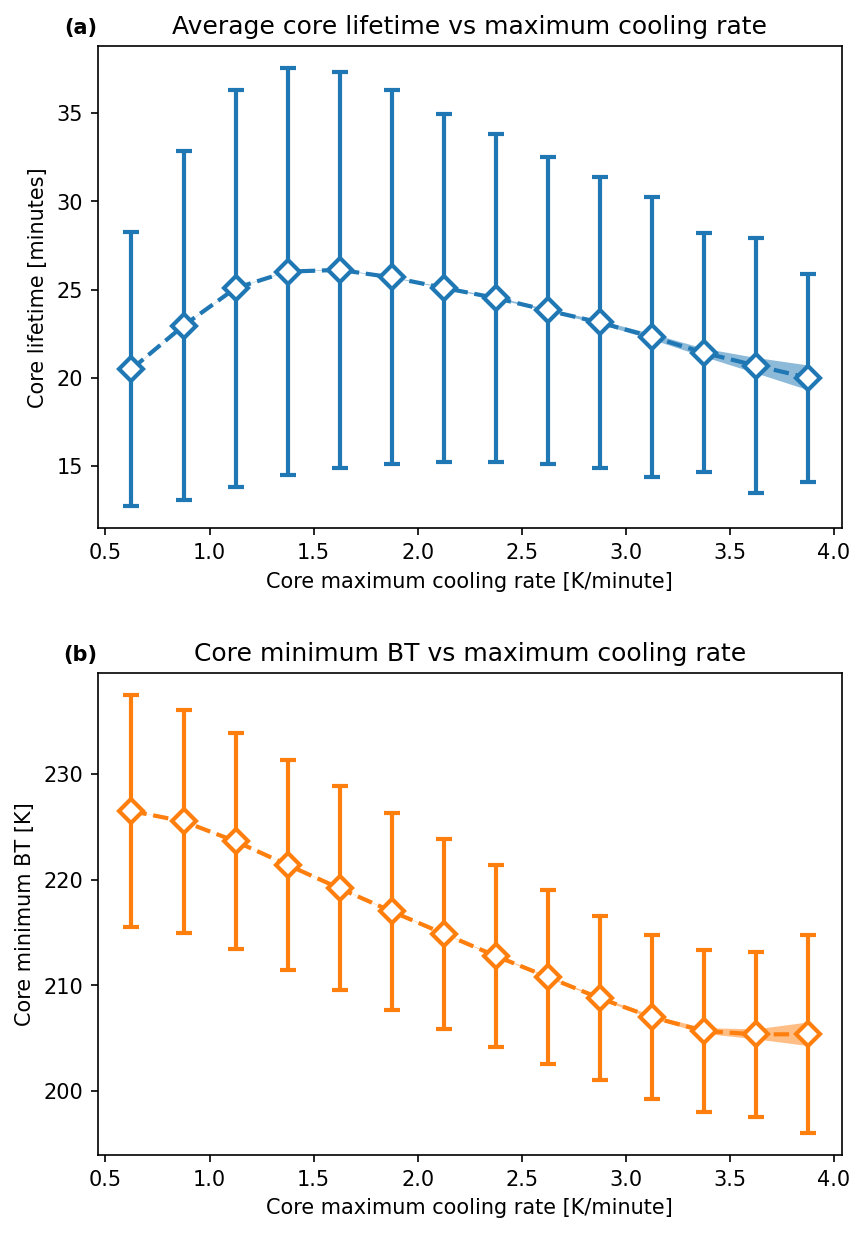
\includegraphics[width=0.75\textwidth]{figures/ch2_10.png}
    \caption[
    Average core lifetime and minimum \acrshort{bt} with increasing core cooling rate
    ]{
    Average core lifetime (a) and minimum \acrshort{bt} (b) with increasing core cooling rate. Error bars show the variance of the data, while the shaded area shows the standard error of the mean.
    }
    \label{fig:core_cooling_rate_relations}
\end{figure}

Figure~\ref{fig:core_cooling_rate_relations}\,b shows how the minimum \acrshort{bt} changes with the maximum cooling rate of the core.
Unlike fig.~\ref{fig:core_cooling_rate_relations}\,a, we see a continuous decrease in \acrshort{bt} with core cooling rate, indicating that faster cooling rates tend to result in cores with colder \acrshort{ctt} and hence higher \acrshort{cth}.
Figure~\ref{fig:core_cooling_rate_relations}\,b also provides context for the results seen in fig.~\ref{fig:core_cooling_rate_relations}\,a.
If we assume that cores are detected around the freezing level (273\,\unit{K}), then we see that the overall temperature change over the core lifetime ranges from $\sim$45\,\unit{K} for the least intense cores to $\sim$65\,\unit{K} for the most intense cores.
Although this continues to increase with cooling rate, the proportional change is less than that of the core cooling rate itself.
As we can approximate the core lifetime as the core \acrshort{bt} change divided by the cooling rate, the larger proportional change in cooling rate will result in a shorter lifetime for more rapidly cooling cores.

%f
\begin{figure}[tp]
    \centering
    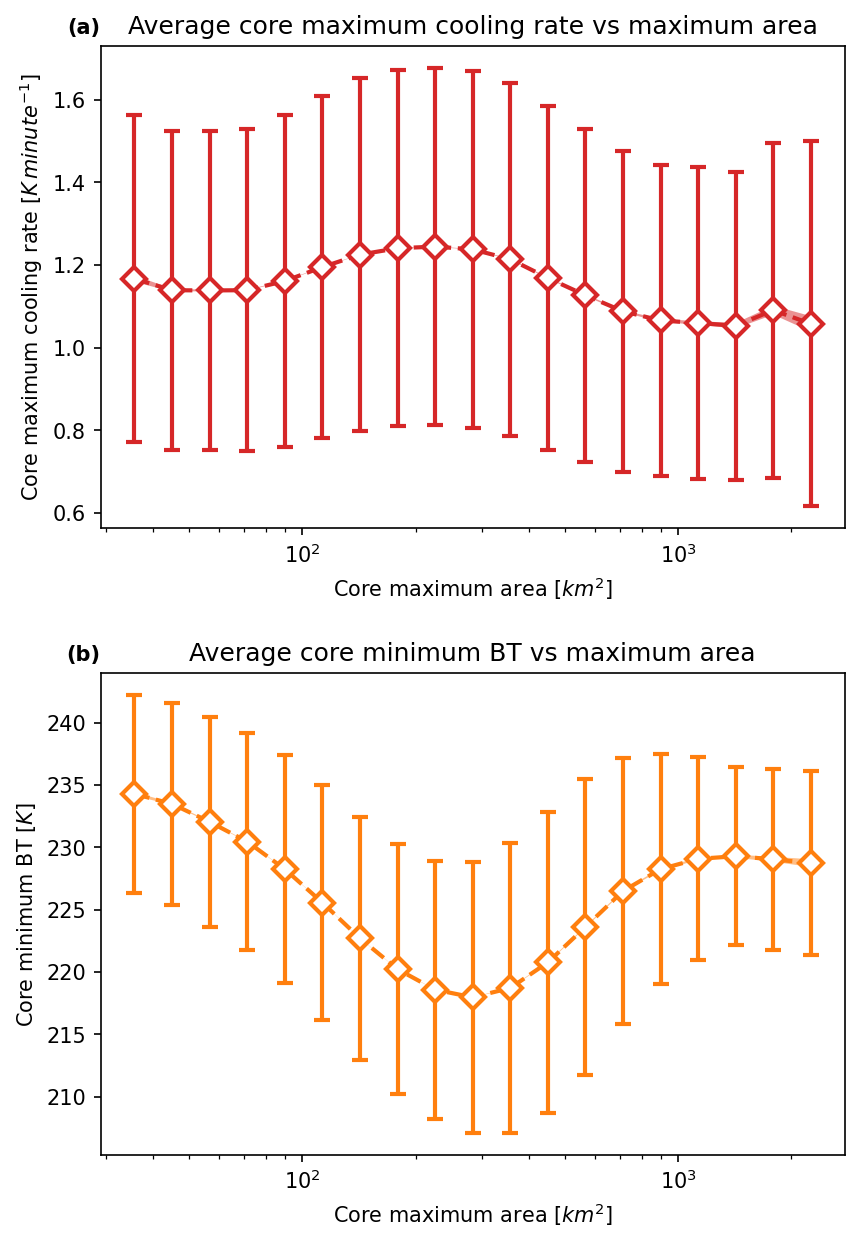
\includegraphics[width=0.75\textwidth]{figures/ch2_11.png}
    \caption[
    Average core cooling rate and minimum \acrshort{bt} with increasing maximum area
    ]{
    Average core cooling rate (a) and minimum \acrshort{bt} (b) with increasing maximum area. Error bars show the variance of the data, while the shaded area shows the standard error of the mean.
    }
    \label{fig:core_area_relations}
\end{figure}

Figure~\ref{fig:core_area_relations} shows how core properties change with the maximum area of the core.
Core area is important for core development, as it influences the amount of entrainment of surrounding air during the growth of the core.
This entrainment has a greater effect on cores with smaller area, and may reduce the maximum height of the core.
We see an increase in average core cooling rate (fig.~\ref{fig:core_area_relations}\,a) and a decrease in minimum \acrshort{bt} (fig.~\ref{fig:core_area_relations}\,b) with core maximum area up to areas of around 250\,\unit{km}, indicating an increase in core growth with increasing area.
Beyond this, however, we see a decrease in cooling rates and an increase in minimum \acrshort{bt} with increasing area, indicating a weakening of convective growth.
It is possible that for these very large regions of growing \acrshort{dcc}, we see a dilution in the vertical ascent due to it being spread over such a large area.
% In fig. \ref{fig:sea_breeze_effect} we explicitly show this relationship by plotting the mean time of core detection against distance from the coast.
% We see a clear trend towards an earlier time of detection as the distance to the coast reduces, indicative of a sea breeze effect.
% The maximum extent of the sea breeze effect extends to between approximately 200\,\unit{km}, similar to the extent of the sea breeze effect quantified using models over the Congo \citep{park_environmental_2020}.

% %f
% \begin{figure}[tp]
%     \centering
%     \includegraphics[width=\textwidth]{sea_breeze_effect.png}
%     \caption{The mean time of detection for observed cores, binned into 25~km intervals of the distance between the location of core initiation and the nearest coastline. A clear trend towards an earlier time of initiation closer to the coast can be seen, with the time of initiation increasing up to approximately 200~km from the nearest coastline.}
%     \label{fig:sea_breeze_effect}
% \end{figure}

% To further investigate the differences in observed core properties across North America, we classify observed cores into four regions shown in fig. \ref{fig:regions}.
% These four regions were selected due to the observed behaviours of cores seen in previous figures.
% The ocean region contains all cores detected over the Gulf of Mexico, the Caribbean and the Western Atlantic.
% The coastal region is defined as the areas within 250~km of the ocean region, chosen to investigate the sea-breeze affected areas demonstrated by fig. \ref{fig:sea_breeze_effect}.
% The inland areas are further divided into two regions.
% Firstly, the Great Plains, to investigate the areas with increased anvil lifetime and later time of detection as seen in figures \ref{fig:core_lifetime_map} and \ref{fig:core_detection_time_map} respectively.
% Secondly, the Midwest, in contrast to the Great Plains region, represents more typical over-land convection seen in the dataset.

% %f
% \begin{figure}[tp]
%     \centering
%     \includegraphics[width=\textwidth]{regions_classification.png}
%     \caption{Observations are classified into four regions for further analysis, based on the differences observed in previous figures. Note that the same colours will be used to refer to each region in all subsequent figures. The black dashed line shows the Western limit of observations for the dataset, with no observations recorded further West than this.}
%     \label{fig:regions}
% \end{figure}

% %f
% \begin{figure}[tp]
%     \centering
%     \includegraphics[width=\textwidth]{regions_initiation_dist.png}
%     \caption{Histograms of core time of detection frequency for each of the four regions in fig. \ref{fig:regional_tod}. Core time of initiation is binned into hour intervals.}
%     \label{fig:regional_tod}
% \end{figure}

% Figure \ref{fig:regional_tod} shows the distributions of time of day of detection for cores observed within each of the regions shown in fig. \ref{fig:regions}.
% The distributions of initiation time for cores over the ocean show a noticeably different distribution to those over land.
% The diurnal variation over the ocean is much weaker, however there is still a peak in the morning (and a corresponding low point in the evening) as seen by the average time of initiation in fig. \ref{fig:regional_tod}, which is again explained due to convective initiation being triggered by night-time cooling of the upper atmosphere through longwave emissions.

% Over land, we see the highest frequency of cores detected in the coastal region, agreeing with the distributions shown in fig. \ref{fig:core_density_by_season}.
% In addition, we see an earlier maximum in the diurnal cycle of 13:00-14:00, compared to that of the Midwest and Great Plains regions of 14:00-15:00.
% This agrees with the impact of the sea breeze shown in fig. \ref{fig:sea_breeze_effect}.

% Comparing the diurnal cycle of core detection between the Midwest and Great Plains region, we see that the Great Plains region shows a greater frequency of detected cores outside of the peak time period in the afternoon.
% In particular, we see increased rates of core detection in the early evening compared to the Midwest region, which is possibly indicative of the bimodal diurnal cycle of deep convection seen previously over the northern great plains \citep{feng_spatiotemporal_2019, li_high-resolution_2021}.

% %f
% \begin{figure}[tp]
%     \centering
%     \includegraphics[width=\textwidth]{regions_lifetime_dist.png}
%     \caption{The frequency distributions of observed core lifetimes for each region, binned by 5 minute intervals.}
%     \label{fig:region_core_lifetimes}
% \end{figure}

% %f
% \begin{figure}[tp]
%     \centering
%     \includegraphics[width=\textwidth]{regions_cooling_rate_dist.png}
%     \caption{The frequency distributions of the maximum cooling rate detected within each core -- which corresponds to the growth rate of the core -- for each region. Binned by 0.1~K/minute intervals.}
%     \label{fig:region_cooling_rate}
% \end{figure}

% In fig. \ref{fig:region_core_lifetimes} and fig. \ref{fig:region_cooling_rate} we see the distributions of core lifetime and maximum core cooling rate respectively for each of the regions.
% The distribution of core lifetimes shows little difference between each region, with the Great Plains having a marginally longer tail.
% The distribution of core cooling rates again shows little difference between each region, however there is a more noticeable increase in the frequency of higher cooling rates over the Great Plains, indicative of more intense convection in the region.


% \section{Observed trends in core behaviour}



% %f
% \begin{figure}[tp]
%     \centering
%     \includegraphics[width=\textwidth]{core_lifetime_vs_tod.png}
%     \caption{}
%     % \label{fig:detected_anvils}
% \end{figure}


% %f
% \begin{figure}[tp]
%     \centering
%     \includegraphics[width=\textwidth]{core_lifetime_vs_cooling_rate.png}
%     \caption{The mean core lifetime for each region, grouped by the maximum core cooling rate in 0.1~K/minute intervals.}
%     \label{fig:lifetime_vs_tod}
% \end{figure}



\subsection{Distributions and properties of observed anvil clouds} \label{sec:anvil_properties}

In this section, we examine the properties of anvil clouds detected in our dataset.
Anvils are detected and tracked semi-independently from cores.
Although they must be associated with observed cores, we continue tracking the anvils beyond the extent of the observed core lifetime.
This also allows us to detect anvils that are associated with multiple cores, providing insight into the effects of convective organisation.

%f
\begin{figure}[tp]
    \centering
    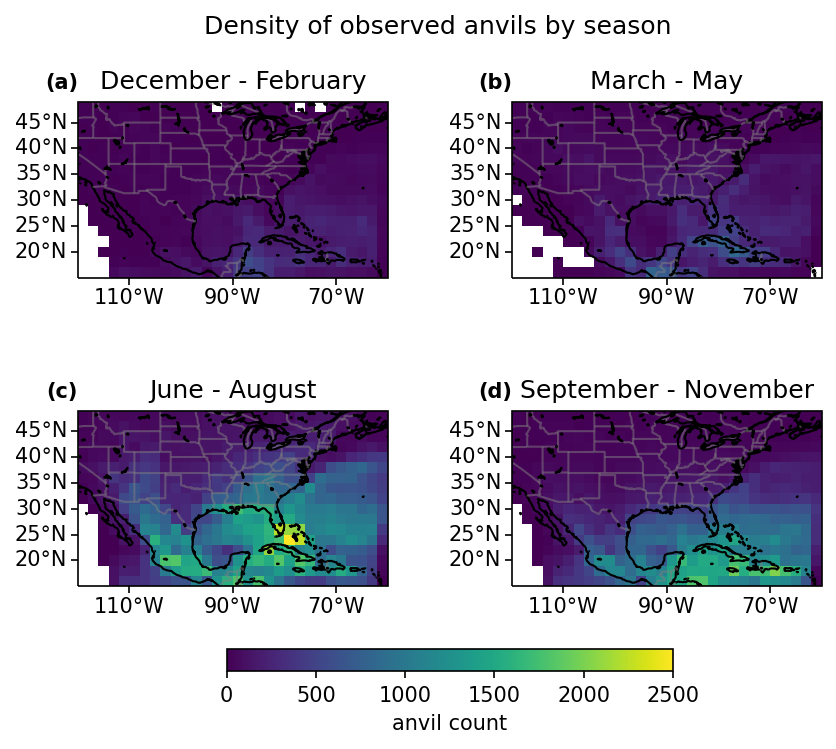
\includegraphics[width=\textwidth]{figures/ch2_12.png}
    \caption[
    The spatial distribution of observed anvils by season
    ]{
    The spatial distribution of observed anvils by season, binned to a 2\texttimes2\,\textdegree grid.
    }
    \label{fig:anvil_distribution_map}
\end{figure}

Figure~\ref{fig:anvil_distribution_map} shows the counts of anvils for each 2\texttimes2\,\textdegree grid box, separated by season.
We see a similar seasonal cycle and distribution to fig.~\ref{fig:core_density_by_season}.
In winter (fig.~\ref{fig:anvil_distribution_map}\,a) and spring (fig.~\ref{fig:anvil_distribution_map}\,b) we see low rates of convection, with the majority of convection observed over warm ocean regions.
In summer (fig.~\ref{fig:anvil_distribution_map}\,c), we see the highest rates of anvil detections, with a large increase in the observations of anvils over land.
In spring (fig.~\ref{fig:anvil_distribution_map}\,d), the number of anvils observed over the ocean remains high, but that over land reduces.

%f
\begin{figure}[tp]
    \centering
    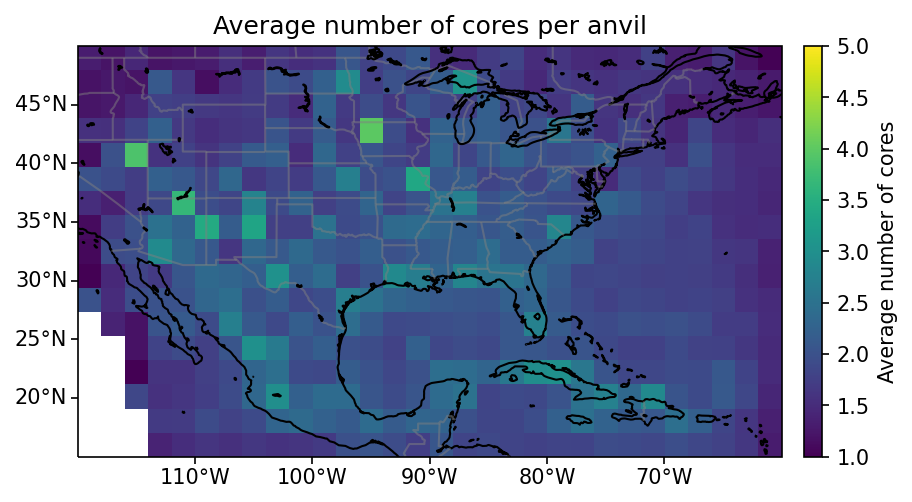
\includegraphics[width=\textwidth]{figures/ch2_13.png}
    \caption[
    The average number of cores associated with each anvil cloud
    ]{
    The average number of cores associated with each anvil cloud, binned to a 2\texttimes2\,\textdegree grid.
    }
    \label{fig:anvil_number_of_cores_map}
\end{figure}

Figure~\ref{fig:anvil_number_of_cores_map} shows the average number of cores associated with each anvil in each 2\texttimes2\,\textdegree grid box.
Over the Caribbean, we see a noticeable land--sea contrast with an increase in the average number of cores over land, indicating that there is greater organisation of convection occurring there compared to over the sea.
For the majority of land regions the average is reasonably noisy.
This is primarily due to the presence of a small number of very large systems (including \acrshort{mcs}s), which have a very large number of cores and hence introduce noise to the spatial average.
In addition, we see a reduction in the average number of cores towards the edge of the map which is likely due to larger anvils being more likely to be removed from the dataset by the criteria in table~\ref{table:anvil_validity_criteria}.

%f
\begin{figure}[tp]
    \centering
    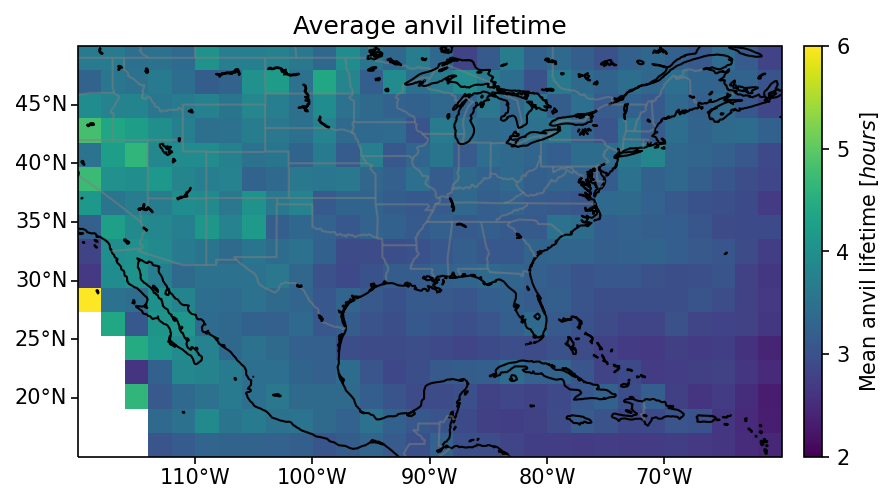
\includegraphics[width=\textwidth]{figures/ch2_14.png}
    \caption[
    The average lifetime of detected anvils
    ]{
    The average lifetime, in hours, of detected anvils, binned to a 2\texttimes2\,\textdegree grid.
    }
    \label{fig:anvil_lifetime_map}
\end{figure}

Figure~\ref{fig:anvil_lifetime_map} shows the average anvil lifetime (in hours) for each 2\texttimes2\,\textdegree grid box.
As in fig.~\ref{fig:anvil_number_of_cores_map}, we see a land--sea contrast in the Caribbean region.


%f
\begin{figure}[tp]
    \centering
    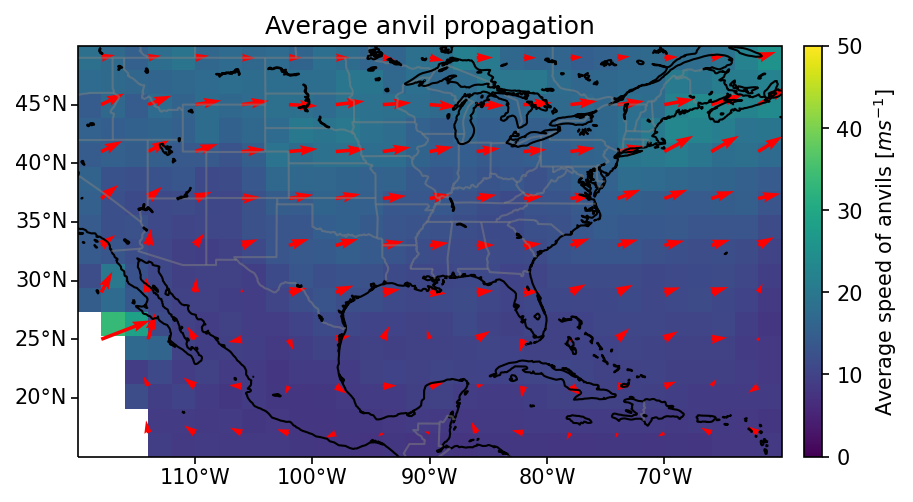
\includegraphics[width=\textwidth]{figures/ch2_15.png}
    \caption[
    The average speed and direction of propagation of anvils
    ]{
    The average speed and direction of propagation of cores observed within each 2\texttimes2\textdegree\ grid box. The colouring shows the average speed of propagation, and the red arrows show the average direction of propagation for each 4\texttimes4\textdegree\ grid box
    }
    \label{fig:anvil_propagation_map}
\end{figure}

Figure~\ref{fig:anvil_propagation_map} shows the average propagation speed and direction for anvils in the same manner as shown for cores in fig.\ref{fig:core_propagation_map}.
Similar to cores, we see a difference in propagation between the tropics and extra-tropics, however the direction and speed of propagation are different in both cases.
Over the tropics (\textless30\,\textdegree\,N), we see no overall average direction of propagation.
In the extra-tropics (\textgreater30\,\textdegree\,N), there is generally an eastward motion, without the northward motion seen in the cores.
The speed of propagation is also slower than that seen for cores, indicating a shear between the two.

%f
\begin{figure}[tp]
    \centering
    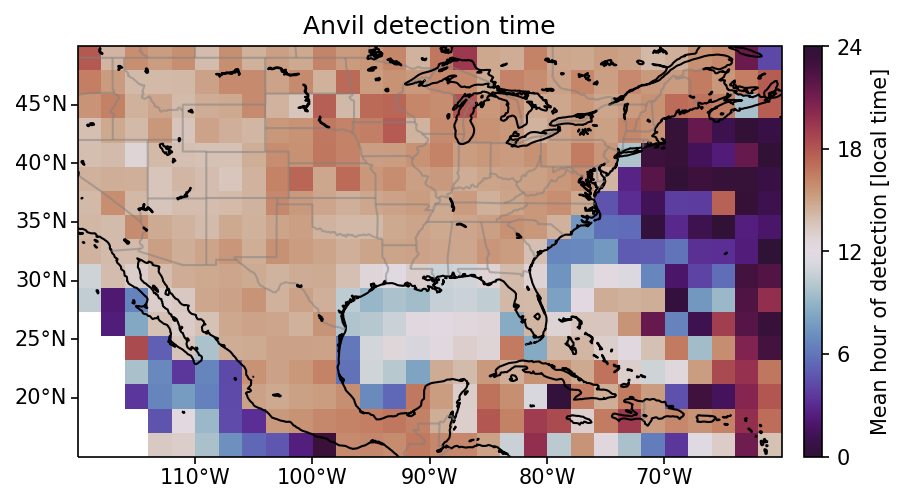
\includegraphics[width=\textwidth]{figures/ch2_16.png}
    \caption[
    The average time of detection of anvils
    ]{
    The average time of day of detection of anvils observed within each 2\texttimes2\textdegree\ grid box, calculated as the circular mean of the local solar time.
    }
    \label{fig:anvil_detection_time_map}
\end{figure}

Figure~\ref{fig:anvil_detection_time_map} shows the average local time of day of anvil detection.
Similar to fig.~\ref{fig:core_detection_time_map} we see a strong land--sea contrast.
However, over much of the Caribbean sea we see that the average time of anvil detection is in the afternoon rather than in the morning.
When considering that in fig.~\ref{fig:cores_with_anvils_map} we saw that only 60--70\% of cores in this region were associated with anvils, indicating that many of the cores occurring during the morning are less likely to produce anvil clouds compared to those in the afternoon.

We also see a later average time of detection of anvils over the \acrshort{ngp} region, however there is less of a contrast seen than that for detected cores.
This indicates that the second peak of core convective activity during the nighttime and early morning in fig.~\ref{fig:core_ngp_contrast} is linked to long-lived, multiple core systems including \acrshort{mcs}s, similar to what was found by \citet{feng_spatiotemporal_2019}.

%f
\begin{figure}[tp]
    \centering
    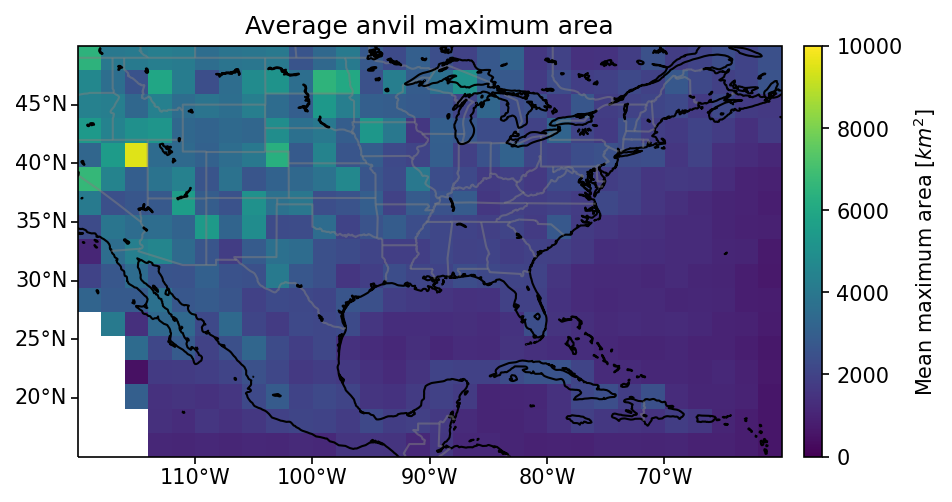
\includegraphics[width=\textwidth]{figures/ch2_17.png}
    \caption[
    The average maximum area of detected anvils
    ]{
    The average maximum area of detected anvils over each 2\texttimes2\textdegree\ grid box
    }
    \label{fig:anvil_area_map}
\end{figure}

Figure~\ref{fig:anvil_area_map} shows the average maximum area of anvils for each 2\texttimes2\,\textdegree grid box.
We again see a land--sea contrast in the Caribbean and Gulf of Mexico.
However, the most notable change is the increase in anvil area as we move towards the North--West of the domain.
This correlates with the change in sensor zenith angle---and hence the area of each pixel---shown in fig.~\ref{fig:abi_zenith_angles}.
It is possible that we are seeing a bias towards observing larger anvils due to the larger pixel area at larger zenith angles.
The large zenith angle may also reduce our ability to detect smaller, isolated \acrshort{dcc}s in these locations. 
However, given the small number of cores and anvils detected in these regions, we do not expect that this will affect our overall statistics.

%f
\begin{figure}[tp]
    \centering
    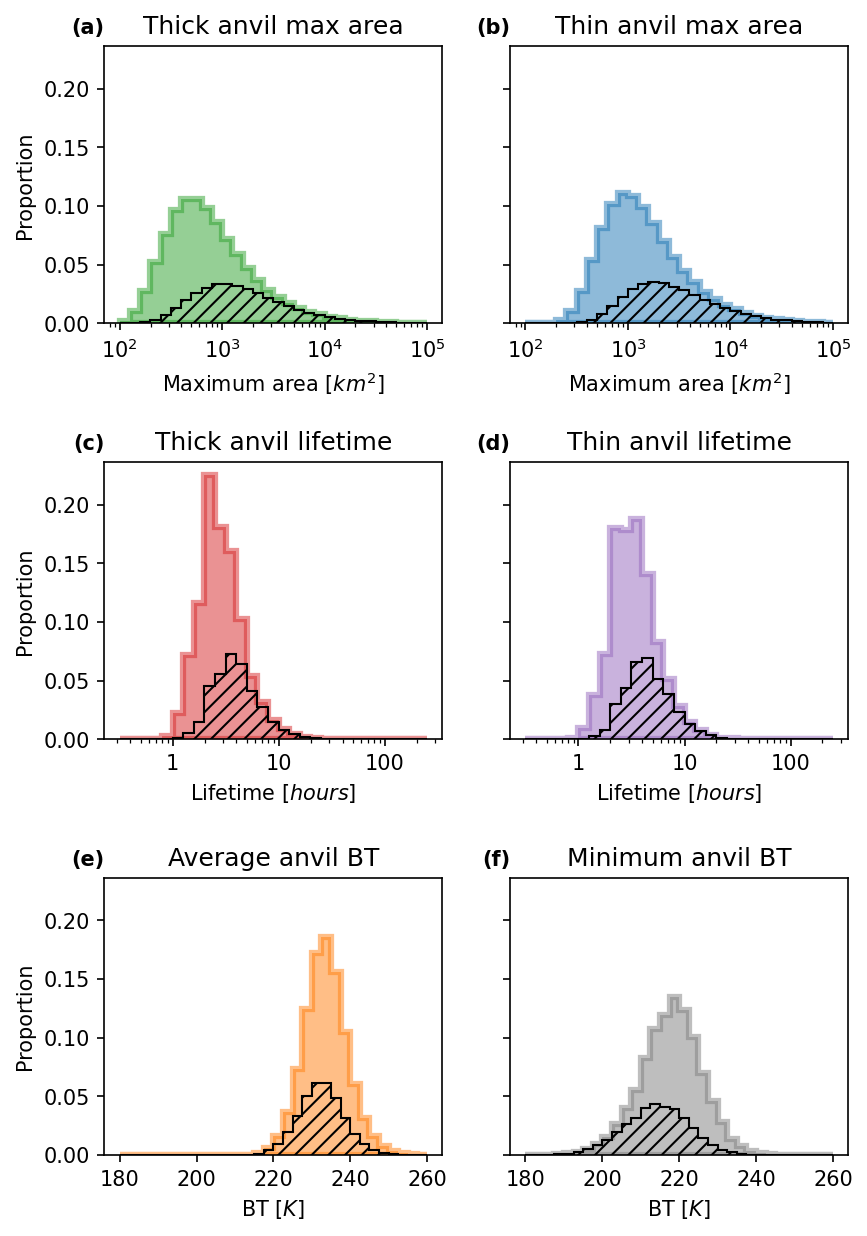
\includegraphics[width=\textwidth]{figures/ch2_18.png}
    \caption[
    The distribution of observed anvil properties
    ]{
    Histograms showing the distribution of observed anvil properties, with the hatched area showing the proportion associated with multiple core anvils. (a) The maximum area of the thick anvil cloud; (b) the maximum area of the thin anvil cloud (which includes both the thick and thin anvil regions; (c) the lifetime of the thick anvil and (d) the thin anvil; and (e) the average and (f) minimum observed \acrshort{bt} within each anvil
    }
    \label{fig:anvil_properties}
\end{figure}

In fig.~\ref{fig:anvil_properties}, we show the distributions of anvil properties, with the proportion consisting of multiple-core anvils shown by the hatched area.
The anvil maximum area distribution has a similar shape for both thick anvils (fig.~\ref{fig:anvil_properties}\,a) and thin anvils (fig.~\ref{fig:anvil_properties}\,b), with the mean shifted to large values for the thin anvil.
It should be noted that the thin anvil area includes that of both thick and thin anvil regions, so will always be larger than that of the thick anvil alone.
The anvil lifetime distributions for the thick (fig.~\ref{fig:anvil_properties}\,c) and thin (fig.~\ref{fig:anvil_properties}\,d) anvils show a similar relationship, with a shift of the distribution to longer lifetimes for the thin anvil.
In both cases, despite the log scaling on the x-axis, we see a longer tail towards larger area values and longer lifetimes.
Furthermore, this large tail consists primarily of multiple-core systems, as shown by the hatched area, indicating the impact of organisation on the area and lifetime of \acrshort{dcc}s.

Figure~\ref{fig:anvil_properties}\,e and fig.~\ref{fig:anvil_properties}\,f show the average and minimum anvil \acrshort{bt} over each detected anvil.
The minimum anvil \acrshort{bt} has a broader distribution than that of the average anvil \acrshort{bt}.
Multiple core anvils generally have colder anvil \acrshort{bt}, particularly so for the minimum \acrshort{bt}.
The cold tail of the minimum \acrshort{bt}, with values less than 200\,\unit{K}, indicates that we may be detecting the presence of overshooting tops within these organised systems.

%f
\begin{figure}[tp]
    \centering
    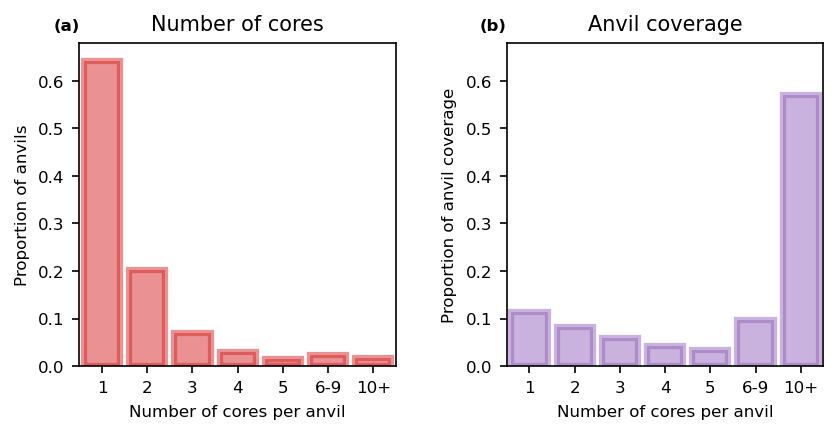
\includegraphics[width=\textwidth]{figures/ch2_19.png}
    \caption{Anvil number of core distribution and coverage}
    \label{fig:anvil_cores_and_coverage}
\end{figure}

Figure~\ref{fig:anvil_cores_and_coverage} shows (a) the distribution of the number of cores associated with each detected anvil, and (b) the proportion of total anvil coverage attributed to anvils with different core counts.
Overall, the vast majority of anvils detected are isolated \acrshort{dcc}s with only a single core.
For anvils with greater than five cores, the number of systems observed drops so low that we have decided to group these into bins of 6--9 cores and 10 or more to ensure that we have a representative sample size.

Despite making up the majority of observed \acrshort{dcc}s, single core systems only make up 12\% of the total anvil coverage.
Instead, despite being few in number, it is the most organised \acrshort{dcc}s---those with ten or more cores---which are responsible for the majority of anvil coverage due to their large area and lifetime.
The large area and lifetime of these systems---seen in the long tails of those distributions in fig.~\ref{fig:anvil_properties}---compound to result in this large coverage.

\subsection{Effects of core intensity and organisation on the lifecycle and thin anvil extent of \acrshort{dcc}s}

Understanding how the structure of anvil clouds changes in response to changes in convective behaviour is vital to understanding climate feedbacks of \acrshort{dcc}s.
Around 50\% of cirrus clouds in the tropics originate from deep convection \citep{massie_distribution_2002, luo_characterizing_2004}.
While the optically thick portion of anvil clouds generally has a neutral effect on the \acrshort{toa} radiative balance, thin cirrus clouds have a strong warming effect.
As a result, changes in convective activity that result in a change in the size of the thin anvil coverage may have large climate feedbacks.

Assessing the extent of thin anvil cirrus is challenging due to the difficulties in observing these clouds using \acrshort{ir} radiometers.
The low emissivity of thin cirrus clouds means that the observed signal is dominated by radiances from the lower atmosphere and surface below.
\citet{protopapadaki_upper_2017} used cloud emissivity and cloud top pressure, rather than \acrshort{bt}, to detect convective cores, thick and thin anvil cirrus clouds.
Data from the AIRS instrument was used to retrieve these emissivity values, as the hyperspectral sounder is more sensitive to thin cirrus than \acrshort{ir} radiometers.
They then compared the proportion of each anvil cloud consisting of thin anvil to the minimum observed cloud top temperature within the convective core, a proxy for the convective depth which is, in turn, a proxy for convective intensity.
It was found that the thin cirrus anvil proportion increased with colder cloud top temperatures, indicating that stronger convection increases the detrainment of thin cirrus.

\citet{takahashi_level_2017} built upon this study using collocated measurements from the \acrshort{cpr} aboard CloudSat.
The \acrshort{cpr} measurements provide the echo top height, measuring the convective depth directly, and also provide another proxy for convective intensity, the echo top distance, which is independent of convective depth \citep{takahashi_characterizing_2014}.
It was again found that the proportion of thin cirrus increased with the echo top height, and also increased with decreasing echo top distance (indicating stronger convection).

It should be noted that both of these studies were performed using observations from polar-orbiting satellites in the A-train, and so do not fully sample the diurnal cycle.
In addition, while both studies consider the maturity of the \acrshort{dcc}s observed, the thin anvil proportion is measured at a single point in time, and so differences in the lifetime of the thick and thin anvil cirrus are not considered.
While observing the thin cirrus anvil is difficult using \acrshort{ir} \acrshort{bt}, we have shown in section \ref{sec:anvil_detection} that by using a combination of \acrshort{bt} differences we are capable of detecting thin cirrus.
Using the dataset of tracked anvils, we can investigate changes in the proportion of thick and thin anvil coverage considering both spatial extent and the lifecycle of the anvil cloud.

%f
\begin{figure}[tp]
    \centering
    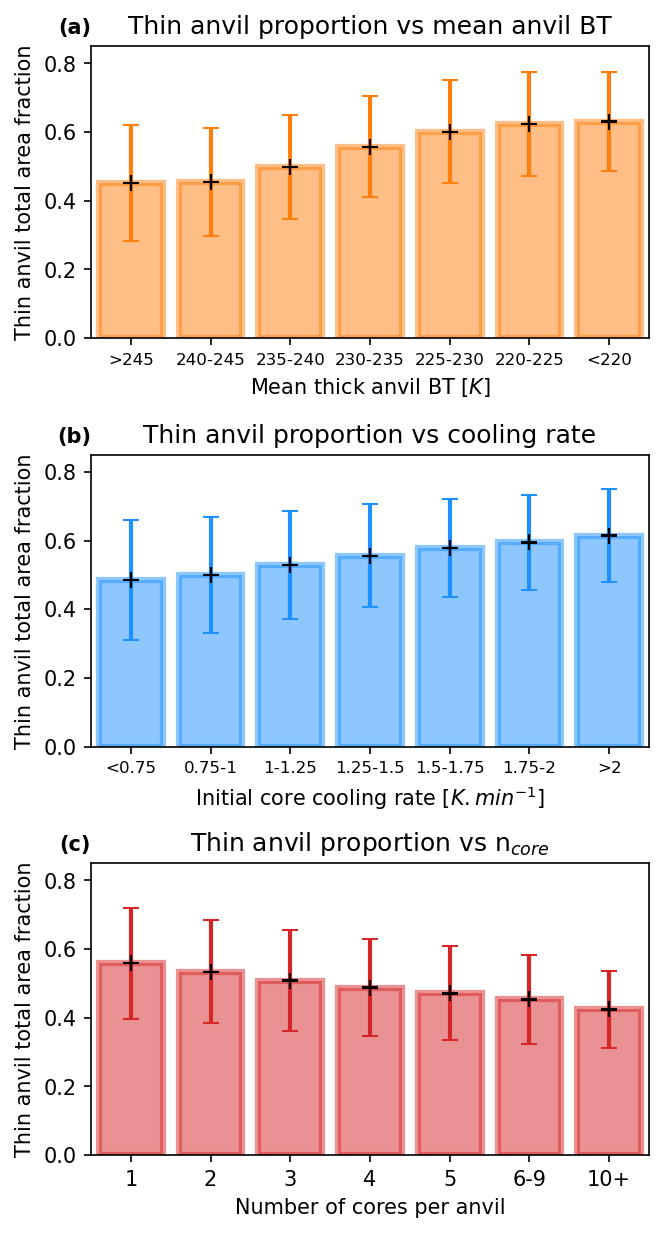
\includegraphics[width=0.75\textwidth]{figures/ch2_20.png}
    \caption{Thin anvil proportion}
    \label{fig:thin_anvil_proportion}
\end{figure}

Figure~\ref{fig:thin_anvil_proportion} shows how the observed thin area proportion of observed anvils changes in regard to observed \acrshort{dcc} properties.
In fig.~\ref{fig:thin_anvil_proportion}\,a we show how the thin anvil proportion changes with the average thick anvil \acrshort{bt} (note here that we only consider the thick anvil \acrshort{bt} to avoid a dependence between the anvil \acrshort{bt} and the thin anvil area).
We see an increase of thin anvil proportion with the average anvil \acrshort{bt}, agreeing with the results of \citet{protopapadaki_upper_2017}.
We see a larger thin anvil fraction compared to \citet{protopapadaki_upper_2017} due to observing the lifetime effects on the thin anvil, rather than comparing a single snapshot of anvil area.

Figure~\ref{fig:thin_anvil_proportion}\,b compares how the thin anvil fraction changes with the maximum cooling rate of the initial core associated with the anvil.
Here we see again that there is a positive relation between the strength of convection and the thin anvil fraction.
This also agrees with the results of \citet{takahashi_level_2017}, who used radar measurements of convective cores to assess the convective strength and its relationship with thin anvil area.

In fig.~\ref{fig:thin_anvil_proportion}\,c, we compare the thin anvil fraction to the number of cores associated with each anvil.
In contrast to fig.~\ref{fig:thin_anvil_proportion}\,b and c, we see a decrease in the thin anvil fraction with an increase in the number of cores.
As this occurs despite the tendency for multiple-core anvils to have colder average \acrshort{bt}, this indicates that further factors are involved in the thin anvil fraction.

In the rest of this section, we will investigate how both the core intensity and organisation impact the lifecycle anvil clouds, and how these changes influence the thin anvil fraction.

%f
\begin{figure}[tp]
    \centering
    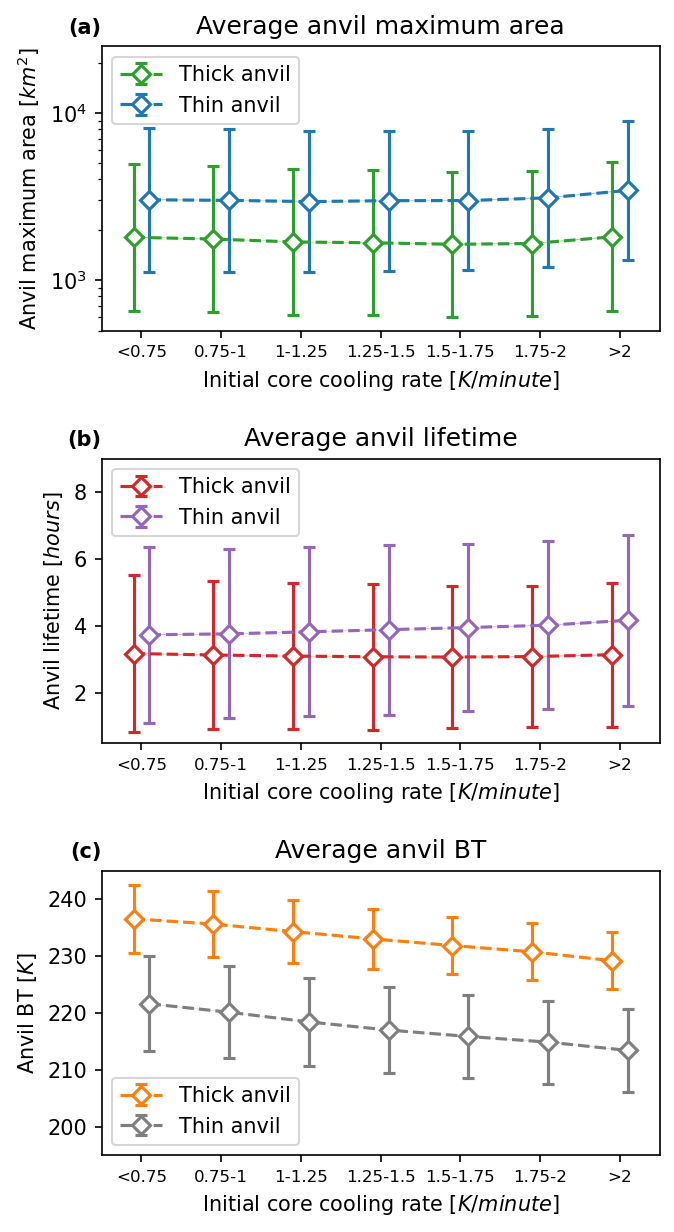
\includegraphics[width=0.75\textwidth]{figures/ch2_21.png}
    \caption{Anvil properties by initial cooling rate}
    \label{fig:anvil_cooling_rate_properties}
\end{figure}

We begin by investigating how the properties of observed anvil clouds change with the maximum cooling rate of their initiating core (that is, the first core observed associated with each anvil).
Figure~\ref{fig:anvil_cooling_rate_properties}\,a shows that the average thick and thin anvil maximum areas vary very little with cooling rate, except for at the highest observed values of cooling rate.
There is however a slight widening in the gap between thick and thin anvil maximum area with increasing core cooling rate.
Figure~\ref{fig:anvil_cooling_rate_properties}\,b shows that while the average thick anvil lifetime remains constant with increasing core cooling rate, the thin anvil lifetime increases.
We also see a consistent decrease in both average and minimum thick anvil \acrshort{bt} with cooling rate, shown in fig.~\ref{fig:anvil_cooling_rate_properties}\,c.


%f
\begin{figure}[tp]
    \centering
    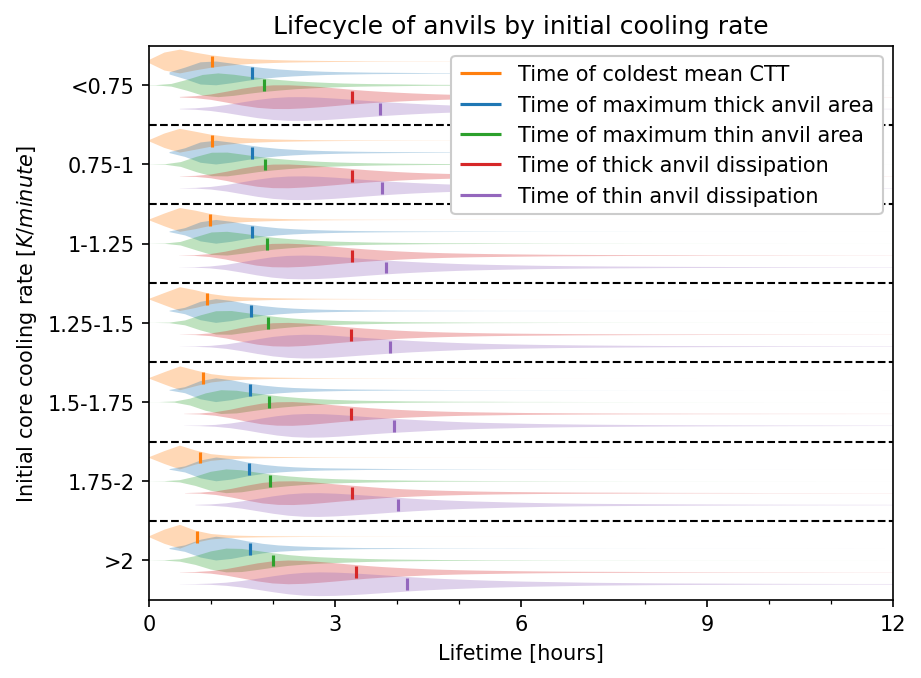
\includegraphics[width=\textwidth]{figures/ch2_22.png}
    \caption{Anvil lifecycle by initial cooling rate}
    \label{fig:anvil_cooling_rate_lifecycle}
\end{figure}

Figure~\ref{fig:anvil_cooling_rate_lifecycle} shows the distribution of the different stages of anvil lifecycle for different bins of initial core cooling rate.
With increasing cooling rate the time of coldest mean \acrshort{bt} becomes earlier, mirroring the findings regarding the relationship between core lifetime and cooling rate found in fig.~\ref{fig:core_cooling_rate_relations}.
While the timing of the maximum thick anvil area and thick anvil dissipation show little change with cooling rate, the time of thin anvil maximum area and dissipation increase.


%f
\begin{figure}[tp]
    \centering
    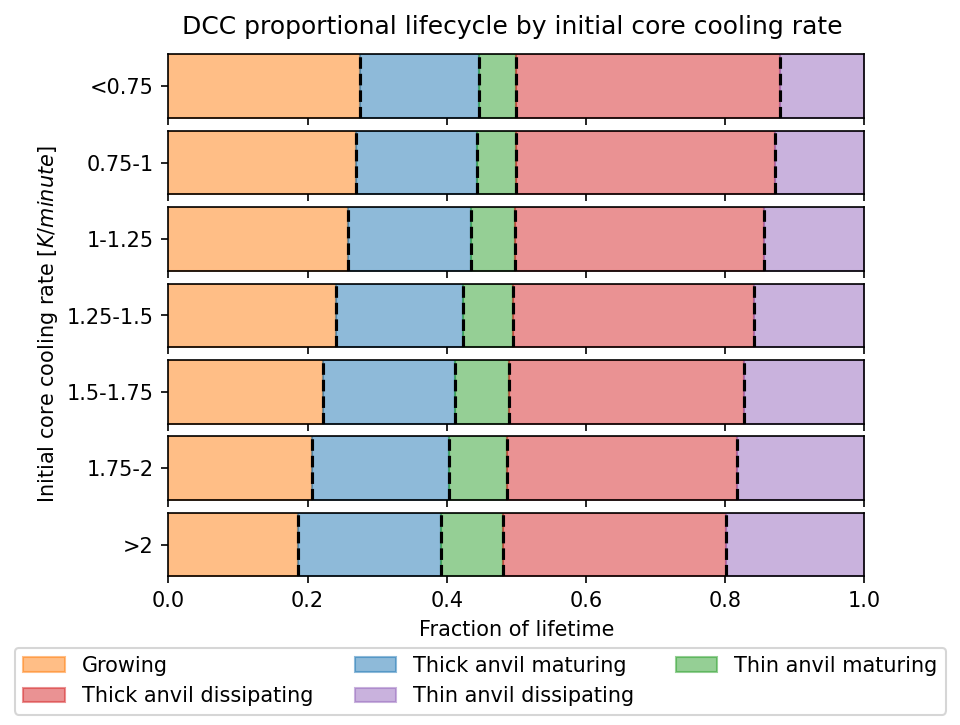
\includegraphics[width=\textwidth]{figures/ch2_23.png}
    \caption{Anvil proportional lifecycle by initial cooling rate}
    \label{fig:anvil_cooling_rate_proportional_lifecycle}
\end{figure}

Figure~\ref{fig:anvil_cooling_rate_proportional_lifecycle} displays the average proportion of anvil lifecycle spent in each of the stages shown in fig.~\ref{fig:anvil_cooling_rate_lifecycle}.
We see again that the primary effect of core cooling rate is to reduce the growing phase and increase the thin anvil dissipation stage.
The thick anvil mature stage remains similar across cooling rate, as does the time between the thick anvil maximum area and thick anvil dissipation.
Overall, this indicates that core cooling rate primarily affects the thin anvil properties, and that the increase in the proportion of thin anvil with cooling rate  is mostly due to an increase in the thin anvil lifetime.

%f
\begin{figure}[tp]
    \centering
    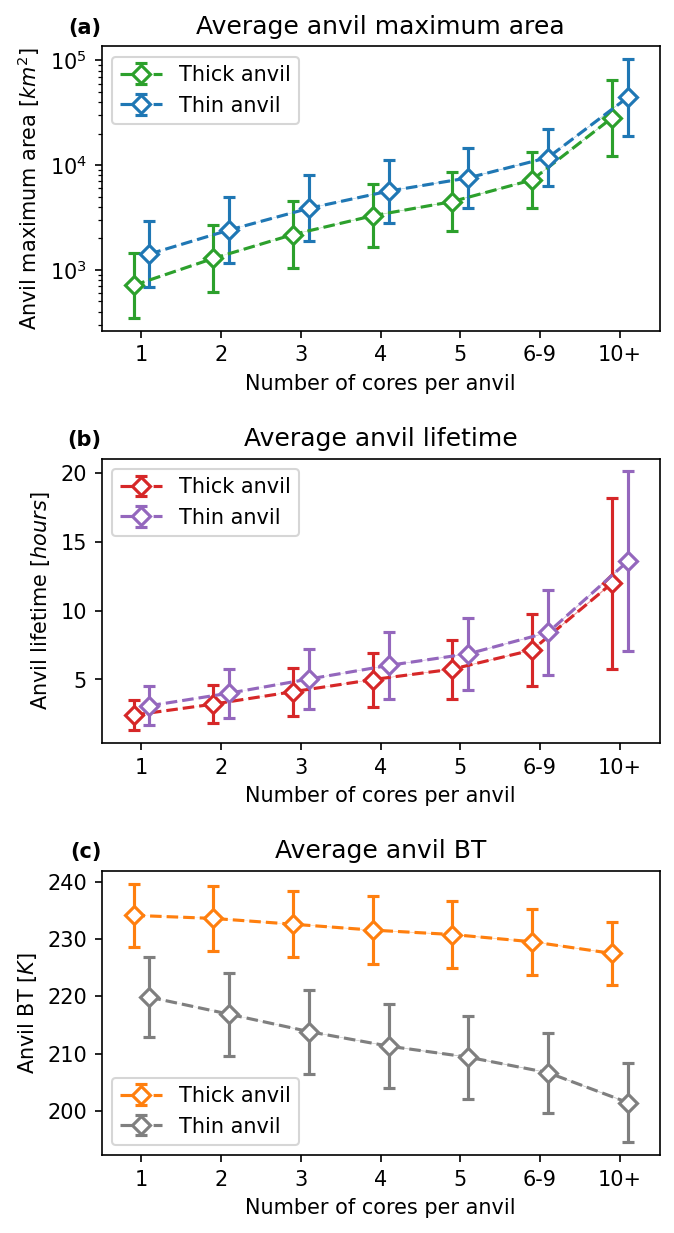
\includegraphics[width=0.75\textwidth]{figures/ch2_24.png}
    \caption{Anvil properties by number of cores}
    \label{fig:anvil_number_of_cores_properties}
\end{figure}

In fig.~\ref{fig:anvil_number_of_cores_properties} we examine how the anvil properties change with the number of cores associated with each anvil cloud.
Figure~\ref{fig:anvil_number_of_cores_properties}\,a shows that both the thick and thin anvil maximum area increase substantially with an increasing number of cores.
However, the thin anvil area increases at a slower rate proportional to the thick anvil.
We see a similar increase in the thick and thin anvil lifetime with increasing number of cores in fig.~\ref{fig:anvil_number_of_cores_properties}\,b.

We see a similar rate of the decrease of average anvil \acrshort{bt} with the number of cores in fig.~\ref{fig:anvil_number_of_cores_properties}\,c as we did in relation to core cooling rate in fig.~\ref{fig:anvil_cooling_rate_properties}\,c.
The minimum anvil \acrshort{bt} decreases at a notably faster rate with increasing number of cores however.
Although this is indicative of an increased likelihood of overshooting cores in more organised \acrshort{dcc}s, we must also note that the larger area of these systems also makes it more likely to observe colder pixels.

%f
\begin{figure}[tp]
    \centering
    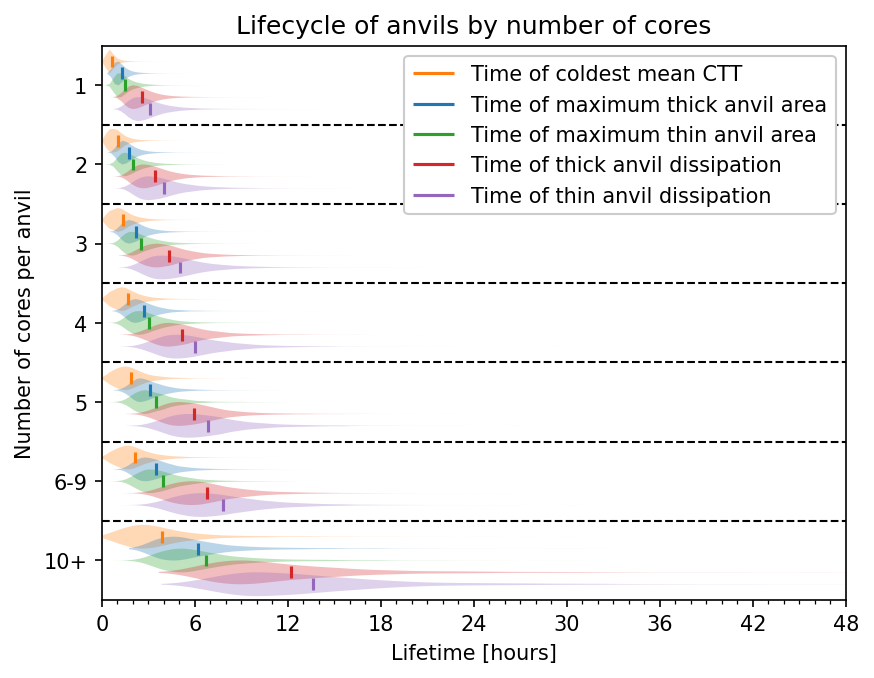
\includegraphics[width=\textwidth]{figures/ch2_25.png}
    \caption{Anvil lifecycle by number of cores}
    \label{fig:anvil_number_of_cores_lifecycle}
\end{figure}

Figure~\ref{fig:anvil_number_of_cores_lifecycle} shows how the timing of the different anvil stages changes with increasing number of cores.
In general, the lifetime of every stage of the \acrshort{dcc} lifecycle increases with the number of cores.
However, the time between the thick and thin anvil maximum area and the thick and thin anvil dissipation increase at a slower rate proportion to the lifetimes of those stages.

%f
\begin{figure}[tp]
    \centering
    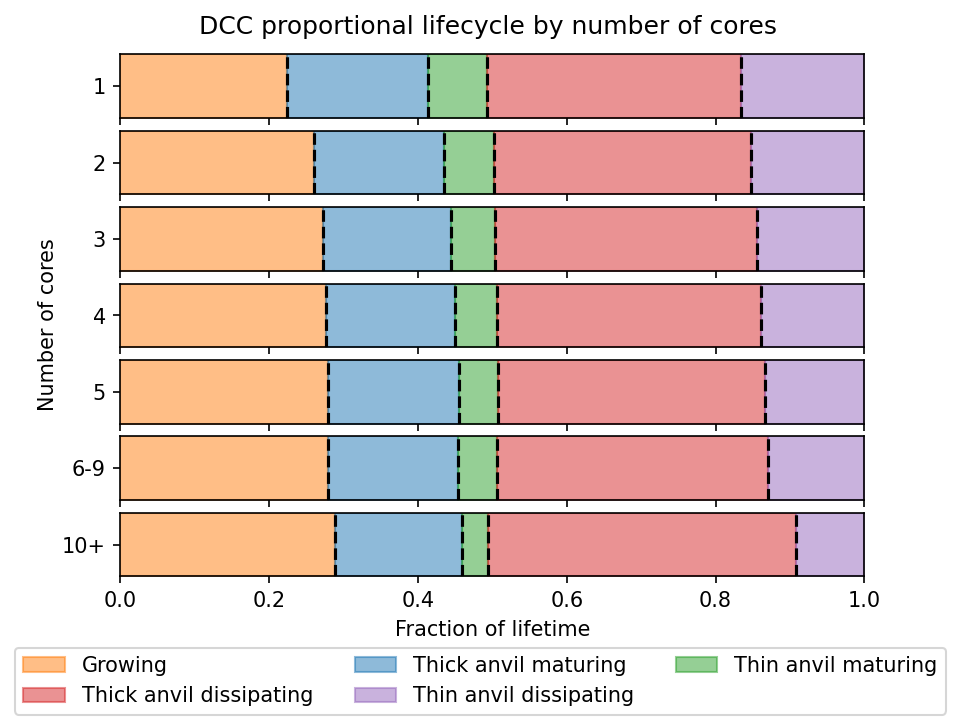
\includegraphics[width=\textwidth]{figures/ch2_26.png}
    \caption{Anvil proportional lifecycle by number of cores}
    \label{fig:anvil_number_of_cores_proportional_lifecycle}
\end{figure}

Figure~\ref{fig:anvil_number_of_cores_proportional_lifecycle} shows the proportion of the overall anvil lifetime spent in the different stages for increasing number of cores, similar to that in fig.~\ref{fig:anvil_cooling_rate_proportional_lifecycle}.
Unlike fig.~\ref{fig:anvil_cooling_rate_proportional_lifecycle}, we see an increase in the growing phase with increasing number of cores, and a decrease in the thin anvil dissipation phase.
In addition, while the thick anvil maturing phase changes little with the number of cores, the time for the thin anvil to reach its maximum area is substantially shorter for \acrshort{dcc}s with the most cores.
It is a combination of the smaller proportional increase in area for the thin anvil, seen in fig.~\ref{fig:anvil_number_of_cores_properties}, and smaller proportion of the \acrshort{dcc} lifecycle spent in the thin anvil dissipating phase which account for the reduction in the thin anvil proportion for increasing number of cores seen in fig.~\ref{fig:thin_anvil_proportion}\,c.

The most interesting result from this comparison is that while the core intensity and \acrshort{dcc} organisation have similar relations to anvil \acrshort{dcc}---the most common proxy used for convective intensity in satellite studies of \acrshort{dcc}s---the have opposite effects on the anvil lifecycle in relation to the thin anvil cirrus.
While \acrshort{dcc}s with individually stronger cores tend to enhance the production and especiall the lifetime of thin anvil cirrus, more organised \acrshort{dcc}s, despite their overall larger area and lifetime, tend to produce a smaller amount of thin anvil in proportion to their thick anvil area.
These two competing effects on thin anvil proportion between two modes of convective intensity may act to control the overall amount of thin anvil cirrus produced by \acrshort{dcc}s.


% %f
% \begin{figure}[tp]
%     \centering
%     \includegraphics[width=\textwidth]{cores_per_anvil_all.png}
%     \caption{Histogram of the frequency of anvils observed by number of cores.}
%     \label{fig:multicore_frequency}
% \end{figure}

% By tracking the anvils associated with detected cores, we can investigate the differences in the properties of anvil clouds in response to changes in the cores.
% Figure \ref{fig:multicore_frequency} show the frequency of anvil clouds detected with different numbers of cores.
% We observe that the majority of anvils form from a single core, with a continuous decay in the number of anvils observed with an increasing number of cores.
% It should be noted however, that as we are detecting cores through observing regions of cooling cloud top temperatures, it is harder to detect cores within mature anvils and as a result we may underestimate the number of cores in larger systems.

% Figure \ref{fig:multicore_fraction_map} shows the fraction of anvils detected that are associated with more than one core in each 1x1 degree grid square.
% There is a noticeable increase in the fraction of multi-core anvils with increasing latitude.
% This is possibly due to the greater influence of large-scale forcing such as the jet stream as we move further from the tropics.

% %f
% \begin{figure}[tp]
%     \centering
%     \includegraphics[width=\textwidth]{multicore_anvil_density.png}
%     \caption{The fraction of anvils observed within each 1x1 degree box that are associated with multiple cores.}
%     \label{fig:multicore_fraction_map}
% \end{figure}

% Figures \ref{fig:anvil_lifetime_by_core} and \ref{fig:thin_anvil_lifetime_by_core} show how the average lifetime of observed anvil clouds varies depending on the number of cores associated with each anvil.
% In both cases, we observe the lifetime of the anvil to increase with the number of cores.
% In general, anvils observed over land have longer lifetimes than those over the coast and ocean.

% %f
% \begin{figure}[tp]
%     \centering
%     \includegraphics[width=\textwidth]{thick_anvil_lifetime_cores.png}
%     \caption{The mean lifetime of observed thick anvil clouds against the number of cores associated with the anvil cloud.}
%     \label{fig:anvil_lifetime_by_core}
% \end{figure}

% Of particular note in fig. \ref{fig:anvil_lifetime_by_core} is the Great Plains region.
% Single-core anvils in this region have short lifetimes similar to those of anvils over the ocean and coast.
% However, the lifetime of anvils over the Great Plains increases more rapidly with the number of cores compared to other regions, and it displays longer lifetimes for multi-core anvils than other regions, potentially indicating greater dynamical interactions.
% In fig. \ref{fig:thin_anvil_lifetime_by_core}, however, we observe that in the Great Plains region the lifetime of the thin anvil cloud for single-core \acrshort{dcc}s is similar to those in the Midwest.
% This indicates that anvils in the Great Plains region have a longer dissipating phase than those of other regions.
% It should also be noted that no significant differences in average core lifetime or growth rates are found for the cores observed associates with multi-core and single-core anvils, so these differences in the anvil behaviour are due to the interactions between multiple cores, not the individual differences in the cores.

% %f
% \begin{figure}[tp]
%     \centering
%     \includegraphics[width=\textwidth]{thin_anvil_lifetime_cores.png}
%     \caption{The mean lifetime of observed thin anvil clouds against the number of cores associated with the anvil cloud.}
%     \label{fig:thin_anvil_lifetime_by_core}
% \end{figure}


\section{Summary}  %% \conclusions[modified heading if necessary]

By producing the first continental scale dataset of both \acrshort{dcc} cores and anvils, we are able to analyse a large number of detected deep convective systems.
We have been able to show a number of key differences in the seasonal, diurnal and regional patterns of \acrshort{dcc}s across the continental \acrshort{usa}.
The spatial distribution of \acrshort{dcc} cores across the continental \acrshort{usa} depends strongly on the seasonal cycle.
The properties of cores themselves, including the lifetime, cooling rate, and time of initiation, have regional dependencies.
We see a large land/sea contrast in time of initiation, and a sea breeze effect which extends for approximately 200\,\unit{km} inland.
In addition, we see differences in the distribution of core time of detection between the two inland regions -- the Midwest and the Great Plains -- with the Great Plains showing a greater spread of convection throughout the night time.
In addition, the Great Plains region shows increased core cooling rates and lifetimes compared to other regions, both of which are associated with more intense convection.
It may be the case that this later time of initiation results in more intense deep convective storms.
The distribution of lifetimes of observed cores shows less difference between different regions, indicating that a number of competing factors may be controlling this property.

While the majority of observed anvil clouds are associated with a single growing core, there remain a large number of multi-core anvils detected in our dataset.
The frequency of multi-core anvils as a proportion of all observed anvils increases with latitude.
Finally, while the properties of the individual growing cores observed in single- and multi-core anvils show no significant difference, the lifetime of anvils clouds shows a large increase with the number of cores.
In addition, the extended lifetime of the thin anvil cloud compared to that of the thick anvil over the Great Plains region may be evidence of the impact of the intensity of convection on the dissipating phase of the \acrshort{dcc}.

Overall, a number of competing factors influence the properties of both \acrshort{dcc} cores and anvils, including the seasonal and diurnal cycles, region, and the number of cores associated with each anvil.
These factors require careful consideration when investigating the response of deep convection to external influences.
Future work will focus on connecting the behaviour of observed \acrshort{dcc}s to meteorological changes including surface temperature, humidity, \acrshort{cape} and \acrshort{cin}, as well as the impact of aerosols on \acrshort{dcc}s.
Furthermore, we will quantify to radiative impacts of anvil clouds across their lifecycle, and aim to investigate the feedbacks of these radiative effects on subsequent convection.

